% CAPÍTULO 4 — RESULTADOS E DISCUSSÃO

\chapter{Resultados e Discussão}
\label{cap:resultados}

Este capítulo apresenta os resultados em três blocos. O primeiro trata da plataforma como artefato de engenharia: o que foi construído, quanto custa consultá-la, se o resultado é reproduzível e como ela opera em nuvem. O segundo relata os achados de qualidade do dado: defeitos encontrados na fonte e um erro de método cometido e corrigido durante o trabalho. O terceiro responde, uma a uma, às cinco perguntas de pesquisa da \autoref{quadro:perguntas}. A ordem do capítulo não é a ordem em que os resultados surgiram: seguindo o ciclo do CRISP-DM, vários deles levaram o trabalho de volta a fases anteriores, e esses retornos estão no \autoref{quadro:crispdm-retornos}.

Todas as tabelas numéricas deste capítulo são geradas a partir dos repositórios públicos de dados (a camada Gold e a listagem das demais camadas) por um \textit{script} do repositório do projeto, e não digitadas. A decisão tem motivo: durante o trabalho, uma lista de códigos mantida à mão passou a divergir do recorte efetivamente aplicado, e o texto afirmou por algum tempo algo que o dado não dizia.

\section{A plataforma construída}

O \textit{pipeline} ingeriu os microdados da RAIS de 2007 a 2025 e do CAGED de 2007 a agosto de 2026. A \autoref{tab:volumes} mostra o volume de cada camada e a \autoref{tab:linhas-camada}, o número de registros dentro do recorte de tecnologia em cada tabela tratada. A Bronze aparece em duas linhas porque o repositório guarda também anos anteriores a 2007 (a RAIS desde 1985), ingeridos mas fora do período analisado; o volume do período é o da primeira linha. A contagem de arquivos não se compara à de uma cópia local, porque 50 arquivos grandes da RAIS foram publicados divididos em 146 partes, com o mesmo conteúdo.

% Gerado por scripts/gerar_tabelas.py --- não editar à mão.
\begin{table}[htbp]
    \centering
    \caption{Volume de cada camada do \textit{data lake}}
    \label{tab:volumes}
    \footnotesize
    \renewcommand{\arraystretch}{1.25}
    \begin{tabular}{lrr}
        \toprule
        \rowcolor{black!8}
        \textbf{Camada} & \textbf{Arquivos} & \textbf{Tamanho} \\
        \midrule
        Bronze, 2007 em diante & 981 & 56,43 GB \\
        Bronze, anos anteriores & 309 & 4,32 GB \\
        Silver de TI & 634 & 1,32 GB \\
        Gold & 29 & < 10 MB \\
        \bottomrule
    \end{tabular}
    \\[4pt]
    Fonte: Autoria própria, a partir da listagem dos repositórios de dados.
\end{table}


% Gerado por scripts/gerar_tabelas.py --- não editar à mão.
\begin{table}[htbp]
    \centering
    \caption{Registros no recorte de tecnologia, por tabela da camada tratada}
    \label{tab:linhas-camada}
    \footnotesize
    \renewcommand{\arraystretch}{1.25}
    \begin{tabular}{lr}
        \toprule
        \rowcolor{black!8}
        \textbf{Tabela} & \textbf{Registros} \\
        \midrule
        \texttt{caged\_mov} & 5.415.877 \\
        \texttt{caged\_old} & 6.268.586 \\
        \texttt{caged\_for} & 100.869 \\
        \texttt{caged\_exc} & 11.283 \\
        \texttt{caged\_ajustes} & 316.799 \\
        \texttt{rais\_vinc} & 23.795.000 \\
        \texttt{rais\_estab} & 2.984.654 \\
        \bottomrule
    \end{tabular}
    \\[4pt]
    Fonte: Autoria própria, a partir da camada Gold.
\end{table}


A redução de volume entre as camadas (\autoref{fig:fluxo-dado}) é o que viabiliza a plataforma: restrito ao recorte de tecnologia, o dado cabe em pouco mais de 1~GB, que se processa em um executor gratuito e se consulta no navegador. O número de arquivos importa tanto quanto o volume: depois da consolidação em um arquivo por partição (\autoref{sec:arquitetura}), uma contagem completa dos vínculos de TI da RAIS passou a responder em 0,4~segundo, lendo apenas os rodapés de metadados dos 19 arquivos da tabela. Em nuvem, a Gold inteira cabe com folga em um executor gratuito: na execução da \autoref{fig:actions}, a etapa mais longa levou 14 minutos. Mais importante que o tempo, a plataforma deixou de depender de uma máquina específica estar ligada, com espaço livre e com as bibliotecas certas funcionando (\autoref{subsec:migracao}).

\section{Reprodutibilidade do recorte}
\label{sec:reprodutibilidade}

A validação mais exigente da plataforma é verificar se o recorte publicado pode ser reconstruído a partir do dado bruto, o que a comparação de agregados com painéis oficiais não garante, porque erros podem se cancelar numa soma. A consulta do \autoref{lst:reprodutibilidade}, no \autoref{apend:consultas}, aplica a definição do recorte ao microdado bruto de junho de 2025 e compara com a camada publicada: são 73.977 movimentações dos dois lados, diferença zero. Como as duas pontas estão publicadas, qualquer pessoa pode repetir a conta. Esse é o sentido de reprodutibilidade adotado aqui: não que o código esteja disponível, mas que a afirmação possa ser recontada da fonte.

Para a RAIS, a verificação cobre todos os anos. Um \textit{script} do repositório aplica a definição do recorte a cada arquivo bruto da Bronze, lendo só as colunas de atividade econômica e de ocupação, e compara a contagem com a camada publicada. O resultado, ano a ano, está na \autoref{tab:reprodutibilidade-rais}, no \autoref{apend:consultas}: diferença zero nos dezenove anos, em 445 arquivos e 23.795.000 registros, inclusive em 2022, já reprocessado. O teste teria apontado a ingestão parcial descrita na \autoref{sec:achados-qualidade} no momento em que ocorreu, porque compara a saída com a fonte, e não apenas a presença de cada arquivo; por isso virou uma etapa do repositório, executável sob demanda no GitHub Actions.

A mesma recontagem foi feita para as cinco tabelas do CAGED, e a \autoref{tab:reprodutibilidade} resume as duas bases: 960 arquivos e 35.908.414 registros, com diferença zero. O resultado, porém, só veio depois de uma correção. A primeira rodada apontou 206.950 linhas a mais no CAGED antigo de 2007, cópias de uma ingestão anterior, com um nome de origem genérico, ao lado das linhas corretas. A duplicata dobrava a série mensal daquele ano e inflava em 26.472 vagas o saldo acumulado do CAGED. A verificação de um mês de 2025, acima, não a encontraria; só a recontagem de todos os anos. Com 2007 reconstruído a partir da Bronze, a diferença é zero em todas as tabelas e anos.

% Gerado por scripts/gerar_tabelas.py --- não editar à mão.
\begin{table}[htbp]
    \centering
    \caption{Recontagem do recorte de tecnologia a partir do dado bruto, por tabela}
    \label{tab:reprodutibilidade}
    \footnotesize
    \renewcommand{\arraystretch}{1.25}
    \begin{tabular}{llrrrr}
        \toprule
        \rowcolor{black!8}
        \textbf{Tabela} & \textbf{Anos} & \textbf{Arquivos} & \textbf{Linhas no dado bruto} & \textbf{Linhas publicadas} & \textbf{Diferença} \\
        \midrule
        \texttt{rais\_vinc} & 2007--2025 & 445 & 23.795.000 & 23.795.000 & 0 \\
        \texttt{caged\_mov} & 2020--2026 & 80 & 5.415.877 & 5.415.877 & 0 \\
        \texttt{caged\_for} & 2020--2026 & 79 & 100.869 & 100.869 & 0 \\
        \texttt{caged\_exc} & 2020--2026 & 77 & 11.283 & 11.283 & 0 \\
        \texttt{caged\_old} & 2007--2019 & 156 & 6.268.586 & 6.268.586 & 0 \\
        \texttt{caged\_ajustes} & 2007--2019 & 123 & 316.799 & 316.799 & 0 \\
        \textbf{Total} &  & 960 & 35.908.414 & 35.908.414 & 0 \\
        \bottomrule
    \end{tabular}
    \\[4pt]
    Fonte: Elaborado pelo autor com dados da RAIS e do CAGED \cite{RAIS2024, CAGED2024}.
\end{table}


\section{Validação contra o painel do MTE}
\label{sec:validacao-mte}

A recontagem a partir do dado bruto mostra que o processamento não perde nem duplica registros, mas não mostra que o recorte conta o que o Ministério contaria. Para isso, os números do trabalho foram comparados com os de um painel público do MTE, publicado em Power BI, cujo modelo traz a RAIS por ocupação e município e o Novo CAGED por ocupação e competência. Relatórios publicados na \textit{web} respondem à mesma interface de consulta que a própria página usa para desenhar os gráficos; um \textit{script} do repositório a consulta filtrando os 34 códigos CBO do recorte de ocupação (com as exclusões e as ocupações avulsas) e compara o resultado com a camada Gold e a Silver.

% Gerado por _utils/validar_painel_mte.py --- não editar à mão.
\begin{table}[htbp]
    \centering
    \caption{Vínculos ativos em 31/12 nas ocupações do recorte: painel do MTE e este trabalho}
    \label{tab:validacao-rais}
    \footnotesize
    \renewcommand{\arraystretch}{1.25}
    \begin{tabular}{lrrrrl}
        \toprule
        \rowcolor{black!8}
        \textbf{Ano} & \textbf{Painel MTE} & \textbf{Trabalho} & \textbf{Diferença} & \textbf{Mediana UF} & \textbf{Faixa nas 27 UFs} \\
        \midrule
        2023 & 862.544 & 869.701 & +0,83\% & +0,92\% & +0,39\% a +4,51\% \\
        2024 & 899.737 & 908.567 & +0,98\% & +1,14\% & +0,51\% a +6,72\% \\
        2025 & 933.962 & 943.890 & +1,06\% & +1,08\% & +0,53\% a +9,18\% \\
        \bottomrule
    \end{tabular}
    \\[4pt]
    Fonte: Autoria própria, a partir do painel público do MTE e da camada Gold.
\end{table}


Na RAIS (\autoref{tab:validacao-rais}), o trabalho conta cerca de 1\% a mais que o painel no total do país, nos três anos que o painel cobre, e a diferença se repete nas 27 unidades federativas: a mediana por estado fica entre 0,9\% e 1,1\%, e as diferenças maiores aparecem só nos estados de estoque muito pequeno, como Roraima, em que poucas dezenas de vínculos pesam vários pontos percentuais.

% Gerado por _utils/validar_painel_mte.py --- não editar à mão.
\begin{table}[htbp]
    \centering
    \caption{Admissões e desligamentos no Novo CAGED nas ocupações do recorte: painel do MTE e este trabalho}
    \label{tab:validacao-caged}
    \footnotesize
    \renewcommand{\arraystretch}{1.25}
    \begin{tabular}{lrrrrrr}
        \toprule
        \rowcolor{black!8}
        & \multicolumn{3}{c}{\textbf{Admissões}} & \multicolumn{3}{c}{\textbf{Desligamentos}} \\
        \rowcolor{black!8}
        \textbf{Ano} & \textbf{Painel} & \textbf{Trabalho} & \textbf{Dif.} & \textbf{Painel} & \textbf{Trabalho} & \textbf{Dif.} \\
        \midrule
        2020 & 204.537 & 206.051 & +0,74\% & 178.727 & 180.354 & +0,91\% \\
        2021 & 325.707 & 327.962 & +0,69\% & 239.337 & 241.038 & +0,71\% \\
        2022 & 304.374 & 307.025 & +0,87\% & 246.016 & 248.389 & +0,96\% \\
        2023 & 237.103 & 240.168 & +1,29\% & 222.630 & 225.106 & +1,11\% \\
        2024 & 251.953 & 255.904 & +1,57\% & 230.201 & 233.462 & +1,42\% \\
        2025 & 267.336 & 271.929 & +1,72\% & 250.589 & 254.475 & +1,55\% \\
        2026 & 172.987 & 176.767 & +2,19\% & 170.738 & 173.332 & +1,52\% \\
        \bottomrule
    \end{tabular}
    \\[4pt]
    Nota: o trabalho inclui as declarações fora do prazo e desconta as exclusões, como o painel. \\
    Fonte: Elaborado pelo autor com dados do painel do MTE \cite{PainelMTE2026} e do CAGED \cite{CAGED2024}.
\end{table}


No Novo CAGED (\autoref{tab:validacao-caged}), a comparação exige um ajuste. O trabalho usa as movimentações informadas no mês; o painel incorpora as declarações fora do prazo e desconta as exclusões, distribuídas pela competência a que se referem. Sem esse ajuste, o trabalho ficava abaixo do painel em 2020 e 2021, anos de muitas declarações tardias, e acima a partir de 2023; com ele, as duas contas passam a diferir entre 0,7\% e 2,2\% em todos os anos, sempre com o trabalho acima (o ano de 2026 vai até agosto).

A diferença tem as três propriedades de uma diferença de critério de contagem, e não de erro de processamento: é pequena, tem sempre o mesmo sinal e se distribui por todas as ocupações e por todos os estados, sem se concentrar em nenhum código ou unidade federativa: na comparação código a código, feita para a RAIS de 2025, nenhuma das 34 ocupações fica abaixo do painel, e as diferenças vão de 0\% a 5,7\%, com mediana de 0,6\%. A documentação pública do painel não permite identificar o critério. Por ser proporcional e estável, a diferença não altera comparações entre anos, estados ou grupos, que são o objeto das cinco perguntas.

A validação tem dois limites. O painel não traz a atividade econômica nas tabelas de fato, e por isso a lente de setor fica sem confronto externo. E a RAIS do painel cobre de 2023 a 2025, o que deixa fora do confronto o ano de 2022, o da ingestão parcial corrigida.

\section{Coerência entre a RAIS e o CAGED}
\label{sec:coerencia-bases}

Se as duas bases medissem o mesmo universo da mesma forma, a variação anual do estoque da RAIS seria igual ao saldo do CAGED no ano. Elas andam juntas, com correlação de 0,97 entre 2008 e 2025, mas não coincidem: no período, o estoque de TI cresceu 841.960 vínculos e o saldo do CAGED somou 662.799, e, em mediana, a variação da RAIS foi 1,24 vez o saldo. É essa razão que o \textit{nowcast} da \autoref{sec:resultado-q5} usa, e saber de onde ela vem diz se o estimador se apoia em uma relação estável ou em um acaso.

A diferença pode ter três origens, e os microdados da RAIS permitem medir cada uma. A primeira é a cobertura: o CAGED registra apenas vínculos regidos pela CLT, e a RAIS inclui estatutários, diretores e contratos temporários. Restrita aos vínculos celetistas, porém, a RAIS ainda cresce 818.104 vínculos, e a diferença quase não muda. As outras duas aparecem quando a variação do estoque celetista é decomposta. Como a RAIS informa, para cada vínculo, o mês de admissão e a situação em 31 de dezembro, a variação se divide, sem resto, em duas parcelas: os vínculos que passam a contar ou deixam de contar como TI sem admissão nem desligamento (troca de ocupação no mesmo empregador, mudança da atividade da empresa, transferência entre estabelecimentos) e as admissões menos os desligamentos registrados na própria RAIS. Só a segunda parcela tem correspondente no CAGED (\autoref{tab:coerencia}).

% Gerado por scripts/gerar_tabelas.py --- não editar à mão.
\begin{table}[htbp]
    \centering
    \caption{Variação do estoque da RAIS e saldo do CAGED, vínculos CLT de TI, 2008--2025}
    \label{tab:coerencia}
    \footnotesize
    \renewcommand{\arraystretch}{1.25}
    \begin{tabular}{lrrrrrrr}
        \toprule
        \rowcolor{black!8}
        \textbf{Período} & \textbf{Var. RAIS} & \textbf{Saldo CAGED} & \textbf{Diferença} & \textbf{Sem contratação} & \textbf{Fluxos} & \textbf{Adm.} & \textbf{Desl.} \\
        \midrule
        2008--2018 & 290.806 & 262.515 & 28.291 & -85.795 & 114.086 & 1,064 & 1,030 \\
        2019--2022 & 394.968 & 307.536 & 87.432 & 126.773 & -39.341 & 1,023 & 1,059 \\
        2023--2025 & 132.330 & 92.748 & 39.582 & 7.410 & 32.172 & 1,020 & 0,995 \\
        \textbf{Total, 2008--2025} & 818.104 & 662.799 & 155.305 & 48.388 & 106.917 & 1,044 & 1,029 \\
        \bottomrule
    \end{tabular}
    \\[4pt]
    Var. RAIS: variação do estoque CLT em 31/12. A diferença para o saldo do CAGED se divide, sem resto, em Sem contratação (vínculos que passam a contar ou deixam de contar como TI sem admissão nem desligamento, inclusive transferências entre estabelecimentos) e Fluxos (admissões menos desligamentos da RAIS, menos o saldo do CAGED). Adm. e Desl.: admissões e desligamentos da RAIS sobre os do CAGED, sem as transferências. Fonte: Elaborado pelo autor com dados da RAIS e do CAGED \cite{RAIS2024, CAGED2024}.
\end{table}


Dos 155.305 vínculos de diferença acumulada, 48.388 (31\%) vêm de mudanças sem contratação, que o CAGED não registra por construção. O sinal dessa parcela muda com o período. Até 2018, ela foi negativa: vínculos deixaram de contar como TI sem desligamento. De 2019 a 2022, somou 126.773 vínculos, no período da migração das declarações para o eSocial e da expansão do setor, quando empregadores passaram a declarar como de TI vínculos que já existiam. É o que explica 2022 ser o pior ano do \textit{nowcast}: o estoque cresceu mais do que o fluxo indicava porque parte do crescimento não passou pelo fluxo.

Os outros 106.917 (69\%) vêm dos próprios movimentos. Sem as transferências, a RAIS registra 4,4\% mais admissões e 2,9\% mais desligamentos que o CAGED no período. A diferença bruta é pequena, mas incide sobre um volume de movimentos cerca de nove vezes maior que o saldo, e por isso pesa no resultado líquido. Ela é compatível com o critério da série do CAGED usada aqui, que conta as movimentações declaradas no prazo e não incorpora as declarações tardias, enquanto a RAIS, anual, recebe o ano completo; é a mesma diferença de critério observada no confronto com o painel do MTE (\autoref{sec:validacao-mte}).

A comparação serviu também como verificação de qualidade. Antes da reingestão do CAGED antigo (\autoref{quadro:achados}), a RAIS registrava de 12\% a 38\% mais admissões que o CAGED entre 2009 e 2014, contra menos de 10\% nos demais anos. A diferença apontava meses em que a extração dos arquivos havia sido interrompida sem erro; com eles reprocessados, as razões desses anos passaram a ficar entre 5\% e 12\%, perto das do restante da série. O que sobra de 2011 tem causa conhecida: o arquivo de março daquele ano está corrompido na própria fonte, e os estados do Sul e do Centro-Oeste estão ausentes do mês. Para o \textit{nowcast}, a conclusão é que a razão histórica não corrige um erro: ela incorpora duas diferenças reais e persistentes de critério entre as bases, e por isso supera a soma direta do fluxo.

\section{Achados de qualidade do dado}
\label{sec:achados-qualidade}

A auditoria descrita na \autoref{sec:auditoria} encontrou defeitos na fonte e um erro de método próprio. Documentá-los é contribuição do trabalho: são obstáculos que qualquer pesquisa sobre as mesmas bases encontrará, e nenhum deles produz mensagem de erro. Cada um foi também um retorno no ciclo do CRISP-DM: detectado na Avaliação ou no Entendimento dos Dados, levou de volta à Preparação ou à Modelagem.

O \autoref{quadro:achados} relaciona os achados. Alguns merecem discussão mais longa pela natureza do problema, e a última subseção mede quanto dado o conjunto deles custou.

\begin{quadro}[htbp]
    \centering
    \caption{Defeitos de dado e de método encontrados durante a construção}
    \label{quadro:achados}
    \footnotesize
    \renewcommand{\arraystretch}{1.3}
    \begin{tabularx}{\textwidth}{%
        >{\raggedright\arraybackslash\hsize=0.70\hsize}X
        >{\raggedright\arraybackslash\hsize=1.35\hsize}X
        >{\raggedright\arraybackslash\hsize=0.95\hsize}X}
        \toprule
        \rowcolor{black!8}
        \textbf{Achado} & \textbf{Descrição} & \textbf{Como foi detectado} \\
        \midrule
        Conversão de salário mínimo invertida & A partir de 2023, um conjunto de registros da RAIS traz a remuneração em salários mínimos com a operação invertida, produzindo valores implausíveis: 222 registros em 2023, 205 em 2024 e 94 em 2025, contra nenhum nos anos anteriores. & Dividir a remuneração nominal pelo salário mínimo do ano e comparar com o valor declarado. \\
        Colunas não harmonizadas & A partir de 2023, arquivos do mesmo ano nomeiam o mesmo campo de formas diferentes, e o sufixo \textit{``\_codigo''} aparece em parte das colunas codificadas. & Comparação de esquema entre arquivos da mesma partição. \\
        Remuneração como texto & Em 2023, sete arquivos trazem a remuneração como texto, e não como número. A verificação por ano não revelava: o esquema agregado do ano mostrava o tipo numérico. & Leitura do esquema \textbf{arquivo por arquivo}. \\
        Código de ocupação não documentado & O código CBO 211220 aparece no microdado com milhares de vínculos ativos, mas não consta de nenhum dicionário oficial do MTE, nem da RAIS, nem do CAGED. & Tradução sem correspondente no dicionário, com código presente no dado. \\
        Domicílio fiscal no lugar do local de trabalho & A localização do vínculo é a do estabelecimento declarante. Municípios com incentivo fiscal aparecem com concentração acima da real. Não é corrigível com o dado público. & Concentração implausível em municípios específicos. \\
        Ingestão parcial de arquivo & Sete pedaços de dois arquivos de 2022 não chegaram à camada tratada: 446.267 vínculos ausentes, cerca de um quarto do ano. & Série anual implausível, e depois verificação pedaço a pedaço contra o bronze. \\
        Duplicata de um ano do CAGED antigo & Em 2007, a camada tinha 206.950 linhas a mais, cópias de uma ingestão anterior que dobravam a série mensal do ano. & Recontagem de todos os anos a partir do dado bruto. \\
        Extração interrompida no CAGED antigo & Em 21 meses de 2008 a 2014, a descompactação parou no meio sem acusar erro, e o mês entrou com parte das linhas: em outubro de 2009, 348 admissões de TI de 21.534. Faltavam 261 mil admissões e 232 mil desligamentos. & Meses muito abaixo dos vizinhos; depois, tamanho extraído conferido com o declarado no próprio pacote, e coerência com a RAIS (\autoref{sec:coerencia-bases}). \\
        Arquivos corrompidos na fonte & Dois arquivos do servidor do MTE falham no teste de integridade, com o mesmo resultado em downloads repetidos: o CAGED antigo de março de 2011, legível só até 55\%, sem PR, SC, RS, MS, MT, GO e DF, e os ajustes de outubro de 2010, com 1\% das linhas. Não é corrigível com o dado público. & Teste de integridade do pacote compactado. \\
        Funcionalismo estadual declarado como programador & O governo de Rondônia declara seus servidores sob um único código CBO, que alterna entre programador de sistemas e operador de máquinas-ferramenta. Nos anos do primeiro, são de 40 a 49 mil falsos profissionais de TI. & Série anual com quedas e saltos implausíveis; depois, um único órgão como maior grupo de TI do país. \\
        Erro de método: Kaplan-Meier em corte transversal & A primeira estimativa de permanência no emprego indicou mediana de 570 meses, ou 48 anos. O estimador pressupõe coorte acompanhada no tempo; a RAIS é corte transversal. & Resultado implausível à inspeção. \\
        Erro de método: mediana agregada por média & A remuneração mediana de um conjunto de grupos foi calculada como a média das medianas dos grupos, ponderada pelo estoque. Em 2025, isso dava 3,55 salários mínimos para o total de TI, contra 3,41 da mediana exata, e invertia a comparação entre as duas lentes. & O mesmo número calculado a partir de duas tabelas de granularidades diferentes (nacional e por UF) deu 3,55 e 3,75. \\
        \bottomrule
    \end{tabularx}
    \\[4pt]
    Fonte: Elaborado pelo autor.
\end{quadro}

\subsection{Ingestão parcial: o limite de uma auditoria por arquivo}

Arquivos grandes da RAIS são processados em pedaços, faixas de linhas alinhadas às bordas dos blocos do Parquet. Em 2022 (ano em que o MTE passou a publicar a RAIS por região, com arquivos muito maiores) sete desses pedaços não chegaram à camada tratada: três do arquivo da região Sul e quatro do de São Paulo. A causa foi uma interrupção de processo durante a regravação desses objetos, que ficaram com metadado de armazenamento truncado, ilegíveis para leitura e recusados para escrita.

A verificação de completude pergunta se cada arquivo-fonte tem saída na camada. Como outros pedaços dos mesmos dois arquivos chegaram, a resposta era afirmativa. O defeito só se tornou visível na série anual: o estoque de 2022 aparecia 14\% abaixo de 2021 e 27\% abaixo de 2023, e o hiato salarial de gênero daquele ano saltava para 29,6\%, contra 6,3\% no ano anterior. Nenhum mercado de trabalho se comporta assim; a implausibilidade da série foi o sintoma.

A correção teve duas partes. A primeira foi reconstruir os pedaços a partir do bronze, o que devolveu os 446.267 vínculos: cada pedaço reconstruído bateu exatamente com a contagem prevista. A segunda, mais importante, foi acrescentar à auditoria uma verificação de completude por pedaço, que recalcula a divisão esperada com a mesma função usada pelo construtor e confronta com a procedência registrada em cada linha da camada. Em \textit{pipelines} que processam arquivos grandes em partes, completude ao nível do arquivo é uma garantia mais fraca do que parece.

\subsection{Funcionalismo estadual declarado como programador}
\label{subsec:artefato-ro}

A série do estoque tinha movimentos que nenhum mercado explicaria: queda em 2011, em plena expansão, salto de 10,8\% em 2018 e estagnação em 2023. Os três vinham do mesmo lugar. Em Porto Velho, o Poder Executivo Estadual de Rondônia declarava entre 40 e 49 mil vínculos ativos com o código CBO 317110, programador de sistemas de informação, em oito anos da série, e entre 0 e 135 nos demais (\autoref{tab:artefato-ro}). Nos anos em que aparecia, esse grupo era o maior conjunto de profissionais de TI do país, maior que o dos desenvolvedores das empresas limitadas da capital paulista.

% Gerado por scripts/gerar_tabelas.py --- não editar à mão.
\begin{table}[htbp]
    \centering
    \caption{Servidores do governo de Rondônia declarados como programador de sistemas}
    \label{tab:artefato-ro}
    \footnotesize
    \renewcommand{\arraystretch}{1.25}
    \begin{tabular}{lrrr}
        \toprule
        \rowcolor{black!8}
        \textbf{Ano} & \textbf{Vínculos ativos do grupo} & \textbf{Estoque de TI sem o grupo} & \textbf{Peso do grupo} \\
        \midrule
        2007 & 40.769 & 519.271 & 7,3\% \\
        2008 & 43.773 & 571.889 & 7,1\% \\
        2009 & 45.173 & 610.240 & 6,9\% \\
        2010 & 48.987 & 665.611 & 6,9\% \\
        2018 & 44.129 & 822.495 & 5,1\% \\
        2019 & 41.352 & 854.478 & 4,6\% \\
        2020 & 43.265 & 899.840 & 4,6\% \\
        2022 & 39.716 & 1.219.223 & 3,2\% \\
        \bottomrule
    \end{tabular}
    \\[4pt]
    Grupo: Poder Executivo Estadual, Porto Velho, CBO 317110. Peso: parcela do estoque de TI que o grupo representaria se não fosse excluído. Fonte: Elaborado pelo autor com dados da RAIS \cite{RAIS2024}.
\end{table}


O dado bruto descarta uma causa histórica. Contando todos os servidores do Executivo estadual em Porto Velho, e não só os do recorte, o total fica estável, entre 45 e 53 mil, e o tempo médio de casa também, entre 140 e 160 meses. O que muda é o código atribuído a quase todos eles: 317110 de 2007 a 2010, de 2018 a 2020 e em 2022, e 721215, operador de máquinas-ferramenta convencionais, de 2011 a 2017. O funcionalismo inteiro do estado aparece, ano a ano, como programador ou como operador de máquinas. Uma mudança real alteraria o número de servidores, e não a ocupação de todos ao mesmo tempo; o padrão é o de um valor padrão no sistema que gera a declaração.

O grupo foi excluído na Gold, nos anos em que passa de mil registros, e permanece na Silver, que continua reproduzindo a fonte. O efeito é grande para um único órgão: o grupo respondia por 7,3\% do estoque de 2007, e retirá-lo elevou o crescimento do período de 143\% para 162\%, levou o hiato salarial de gênero de 2007 de 19,0\% para $-$0,9\%, invertendo a tendência daquela série (\autoref{sec:resultado-q4}), e reduziu o erro médio do \textit{nowcast} de 2,1\% para 1,1\% (\autoref{sec:resultado-q5}). Nenhuma verificação da Silver acusaria o defeito, porque o dado foi lido e traduzido corretamente: o erro está na declaração. A verificação de saltos descrita na \autoref{sec:auditoria} passou a procurar casos assim em toda a série e, hoje, só encontra este.

\subsection{Erro de método: sobrevivência em corte transversal}

A primeira tentativa de medir permanência aplicou o estimador de Kaplan-Meier ao corte transversal da RAIS e produziu mediana de 570 meses, 48 anos de emprego, número absurdo, que expõe a incompatibilidade entre o estimador e a estrutura do dado (\autoref{subsec:sobrevivencia}). A tábua de vida de período troca a pergunta por uma que o dado responde: qual o risco de desligamento em cada faixa de tempo de casa naquele ano. O erro foi detectado por inspeção, e não por um teste automatizado, o que indica onde a validação do trabalho é mais frágil.

\subsection{Erro de método: mediana agregada por média}

Cada tabela da Gold guarda a mediana da remuneração de cada grupo, por exemplo, de cada combinação entre setor e ocupação de TI. Para obter a mediana de um conjunto maior, como o total de TI, a primeira versão do trabalho fez a média das medianas dos grupos, ponderada pelo estoque. O atalho parece razoável e está errado: mediana não se soma, e a média de medianas não é a mediana de nada. O erro só apareceu porque o mesmo número, calculado a partir de duas tabelas com grupos diferentes, não coincidia: para 2025, a tabela nacional dava 3,55 salários mínimos, e a tabela por unidade federativa, 3,75. A mediana exata, calculada sobre os vínculos, é 3,41.

O maior efeito foi sobre uma comparação. Pela média das medianas por setor da empresa, os profissionais de TI que trabalham fora das empresas de TI pareciam ganhar mais que os de dentro; pela mediana exata, ganham menos: 4,13 contra 4,31 salários mínimos em 2025. A Gold passou a guardar a mediana exata dos recortes usados neste texto e a distribuição da remuneração em faixas, da qual o \textit{dashboard} calcula a mediana de qualquer combinação de estados (\autoref{sec:apresentacao}). Todas as medianas deste capítulo vêm dessa versão.

\subsection{Quanto dado se perdeu}
\label{subsec:perdas}

Todo projeto de dados perde parte do que recebe, e o tamanho da perda precisa ser medido, e não presumido. Neste trabalho, ela tem uma única origem. A recontagem a partir do dado bruto (\autoref{sec:reprodutibilidade}) mostrou diferença zero entre o texto publicado pelo MTE e a camada tratada, em todos os anos das duas bases: a extração, a tradução e o recorte não descartam registros. O que se perdeu foi o que a própria fonte não entrega, nos dois arquivos corrompidos do \autoref{quadro:achados}. O pacote compactado declara o tamanho original de cada arquivo, e a extração mede a parte legível; da proporção entre as duas sai a estimativa do que falta (\autoref{tab:perdas}).

\begin{table}[htbp]
    \centering
    \caption{Linhas perdidas nos arquivos corrompidos na fonte}
    \label{tab:perdas}
    \footnotesize
    \renewcommand{\arraystretch}{1.25}
    \begin{tabular}{lrrrl}
        \toprule
        \rowcolor{black!8}
        \textbf{Arquivo} & \textbf{Lidas} & \textbf{No arquivo} & \textbf{Perdidas} & \textbf{Uso nas análises} \\
        \midrule
        CAGED antigo, março de 2011 & 1.880.719 & 3.439.129 & 45,3\% & série mensal, cubos e modelos \\
        Ajustes do CAGED, outubro de 2010 & 1.942 & 192.815 & 99,0\% & nenhum \\
        \midrule
        \textbf{Total, CAGED bruto} & & & \textbf{0,23\%} & 1.749.283 de 769,6 milhões de linhas \\
        \bottomrule
    \end{tabular}
    \\[4pt]
    No arquivo: linhas estimadas pela proporção entre os bytes legíveis e o tamanho original declarado no pacote. Todas as ocupações e setores. Fonte: Elaborado pelo autor com dados do CAGED \cite{CAGED2024}.
\end{table}

Na base inteira, a perda é de cerca de 1,75 milhão de linhas, 0,23\% do CAGED bruto; na RAIS, é nula. No recorte de tecnologia, só o arquivo de março de 2011 importa, porque os ajustes não entram na série nem nos modelos. Como esse arquivo é ordenado por unidade federativa, a perda não é uma amostra: faltam por inteiro Paraná, Santa Catarina, Rio Grande do Sul, Mato Grosso do Sul, Mato Grosso, Goiás e o Distrito Federal, e cerca de metade de São Paulo. Estimando cada estado pela média de fevereiro e abril, corrigida pela sazonalidade de março medida nos estados completos, faltam cerca de 12,1 mil admissões e 8,6 mil desligamentos de TI: 43\% das movimentações do mês, 3,6\% das de 2011 e 0,17\% da série inteira. O saldo de 2011 fica subestimado em cerca de 3,4 mil vagas (40,9 mil observados, contra 44,3 mil estimados), e o saldo acumulado da série, em 0,5\%. A comparação com a RAIS confirma a ordem de grandeza: em 2011, a RAIS registra 12\% mais admissões que o CAGED, contra cerca de 8\% nos anos vizinhos (\autoref{sec:coerencia-bases}).

A série mantém o dado observado, sem imputação. O efeito é pequeno diante das conclusões, que se apoiam em tendências de vários anos, e uma estimativa misturada ao dado observado ficaria indistinguível dele. A lacuna fica declarada aqui e na documentação dos dados publicados.

\section{Pergunta 1: quanto o mercado cresceu}
\label{sec:resultado-q1}

O mercado mais que dobrou em dezoito anos, mas não cresceu de forma contínua: cresceu em ondas. A \autoref{fig:estoque-serie} apresenta a série anual do estoque de vínculos formais de tecnologia e da remuneração mediana em salários mínimos; os valores de cada ano, com o tempo médio de emprego, estão na \autoref{tab:estoque-serie}, no \autoref{apend:series}.

% Gerado por scripts/gerar_tabelas.py --- não editar à mão.
\begin{figure}[htbp]
    \centering
    \caption{Estoque de vínculos formais de TI e remuneração mediana, 2007--2025}
    \label{fig:estoque-serie}
    \begin{minipage}[t]{0.49\textwidth}
    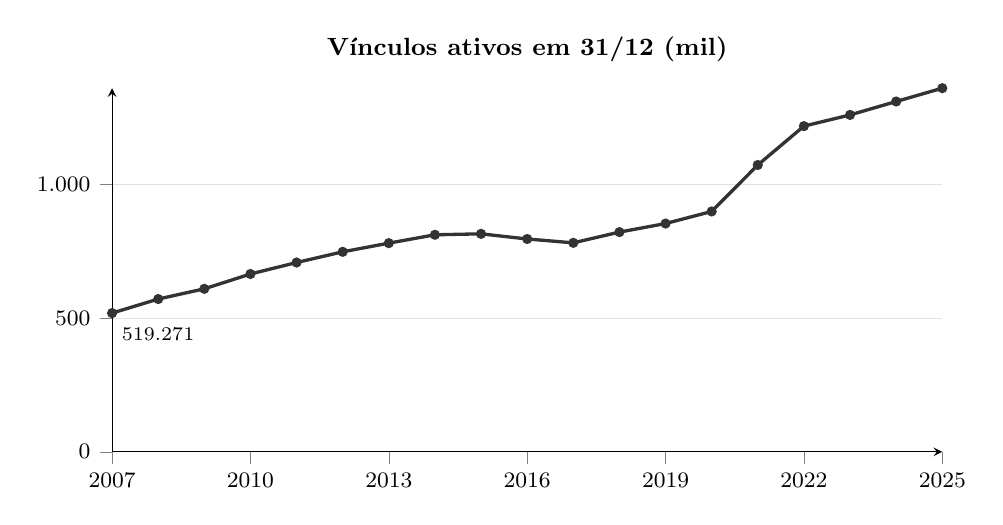
\begin{tikzpicture}
    \begin{axis}[width=\linewidth, height=6.2cm, axis lines=left, tick align=outside,
            ymajorgrids, grid style={black!12}, tick label style={font=\footnotesize},
            label style={font=\footnotesize}, title style={font=\small\bfseries},
            /pgf/number format/use comma, /pgf/number format/1000 sep={.}, title={Vínculos ativos em 31/12 (mil)},
            xmin=2007, xmax=2025, ymin=0, xtick distance=3,
            x tick label style={/pgf/number format/1000 sep={}}]
        \addplot[very thick, black!80, mark=*, mark size=1.2pt] coordinates {(2007,519.3) (2008,571.9) (2009,610.2) (2010,665.6) (2011,708.6) (2012,748.7) (2013,781.2) (2014,812.4) (2015,816.0) (2016,796.7) (2017,782.3) (2018,822.5) (2019,854.5) (2020,899.8) (2021,1073.7) (2022,1219.2) (2023,1261.1) (2024,1311.3) (2025,1361.2)};
        \node[font=\scriptsize, anchor=north west, yshift=-2pt] at (axis cs:2007,519.3) {519.271};
        \node[font=\scriptsize, anchor=south east] at (axis cs:2025,1361.2) {1.361.231};
    \end{axis}
    \end{tikzpicture}
    \end{minipage}\hfill
    \begin{minipage}[t]{0.49\textwidth}
    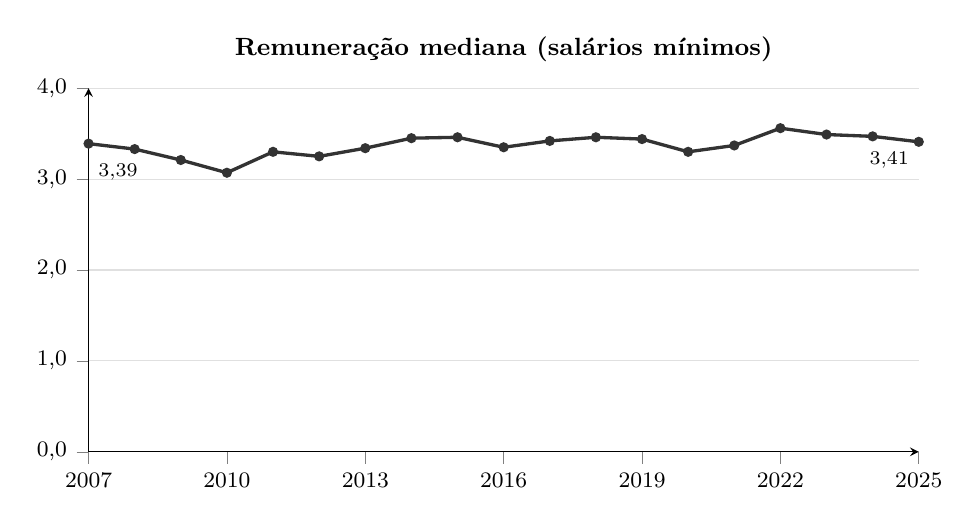
\begin{tikzpicture}
    \begin{axis}[width=\linewidth, height=6.2cm, axis lines=left, tick align=outside,
            ymajorgrids, grid style={black!12}, tick label style={font=\footnotesize},
            label style={font=\footnotesize}, title style={font=\small\bfseries},
            /pgf/number format/use comma, /pgf/number format/1000 sep={.}, title={Remuneração mediana (salários mínimos)},
            xmin=2007, xmax=2025, ymin=0, ymax=4, xtick distance=3,
            x tick label style={/pgf/number format/1000 sep={}},
            y tick label style={/pgf/number format/.cd, use comma, fixed, fixed zerofill, precision=1}]
        \addplot[very thick, black!80, mark=*, mark size=1.2pt] coordinates {(2007,3.39) (2008,3.33) (2009,3.21) (2010,3.07) (2011,3.3) (2012,3.25) (2013,3.34) (2014,3.45) (2015,3.46) (2016,3.35) (2017,3.42) (2018,3.46) (2019,3.44) (2020,3.3) (2021,3.37) (2022,3.56) (2023,3.49) (2024,3.47) (2025,3.41)};
        \node[font=\scriptsize, anchor=north west, yshift=-4pt] at (axis cs:2007,3.39) {3,39};
        \node[font=\scriptsize, anchor=north east] at (axis cs:2025,3.41) {3,41};
    \end{axis}
    \end{tikzpicture}
    \end{minipage}
    \\[4pt]
    {\footnotesize Valores anuais na \autoref{tab:estoque-serie}, no \autoref{apend:series}. }Fonte: Autoria própria, a partir da camada Gold.
\end{figure}


O estoque passou de 519.271 vínculos em 2007 para 1.361.231 em 2025, crescimento de 162\% em dezoito anos, a uma taxa média de 5,5\% ao ano, ritmo que dobra o estoque a cada treze anos. A média, porém, junta fases opostas, separadas na \autoref{tab:fases}.

% Gerado por scripts/gerar_tabelas.py --- não editar à mão.
\begin{table}[htbp]
    \centering
    \caption{Ritmo do crescimento do estoque de TI, por fase}
    \label{tab:fases}
    \footnotesize
    \renewcommand{\arraystretch}{1.25}
    \begin{tabular}{llrrr}
        \toprule
        \rowcolor{black!8}
        \textbf{Período} & \textbf{Fase} & \textbf{Ritmo anual} & \textbf{Vínculos ganhos} & \textbf{Parcela do crescimento} \\
        \midrule
        2007--2014 & Expansão & 6,6\% & 293.146 & 35\% \\
        2014--2017 & Recessão & -1,3\% & -30.108 & -4\% \\
        2017--2020 & Retomada & 4,8\% & 117.531 & 14\% \\
        2020--2022 & Aceleração pós-pandemia & 16,4\% & 319.383 & 38\% \\
        2022--2025 & Desaceleração & 3,7\% & 142.008 & 17\% \\
        \textbf{2007--2025} & \textbf{Período inteiro} & \textbf{5,5\%} & \textbf{841.960} & \textbf{100\%} \\
        \bottomrule
    \end{tabular}
    \\[4pt]
    Ritmo anual: taxa composta de crescimento do estoque em 31/12. Fonte: Autoria própria, a partir da camada Gold.
\end{table}


A expansão até 2014 foi interrompida pela recessão de 2015--2016: entre 2014 e 2017 o setor perdeu 30 mil vínculos, na única fase de queda da série. A retomada a partir de 2017 ganhou velocidade em 2021 e 2022, na aceleração digital que seguiu a pandemia de COVID-19: nesses dois anos o estoque cresceu 19,3\% e 13,6\%, e essa fase sozinha responde por 38\% de todo o crescimento dos dezoito anos. Depois dela o ritmo caiu para 3,7\% ao ano, abaixo da média do período. Esse desenho só aparece depois da correção do artefato de Rondônia (\autoref{subsec:artefato-ro}): com o funcionalismo estadual contado como programador, a série mostrava queda em 2011, salto em 2018 e estagnação em 2023, movimentos que não aconteceram no mercado.

Os números são coerentes com os da literatura (\autoref{sec:relacionados}), com diferenças que o recorte explica. Entre 2012 e 2022, a lente de ocupação deste trabalho cresceu 65\%, contra 95\% medidos pela FECOMERCIOSP para 30 ocupações de tecnologia \cite{Fecomercio2024}: o sentido e a ordem de grandeza coincidem, e a distância é compatível com listas de ocupações diferentes: a seleção por família, as exclusões e a inclusão dos estatísticos mudam a base de comparação. Já os 2,1 milhões de empregos que a BRASSCOM atribui ao macrossetor TIC em 2024 \cite{Brasscom2024} superam o 1,31 milhão deste trabalho porque o macrossetor soma às atividades de TI as de telecomunicações e de equipamentos, fora do recorte adotado aqui.

O fluxo mensal do CAGED confirma e detalha esse desenho. A série construída cobre 236 meses, de janeiro de 2007 a agosto de 2026, com saldo acumulado de 698.951 vagas líquidas. A diferença entre esse acumulado e a variação do estoque da RAIS no mesmo período não é erro: decorre de diferenças de cobertura e de critério entre as bases, medidas na \autoref{sec:coerencia-bases}, e é o que o estimador de \textit{nowcast} da \autoref{sec:resultado-q5} precisa modelar.

\section{Pergunta 2: onde está o trabalho de TI}
\label{sec:resultado-q2}

Esta é a pergunta cuja resposta mais se afasta do senso comum sobre o setor, e é o achado central do trabalho.

% Gerado por scripts/gerar_tabelas.py --- não editar à mão.
\begin{table}[htbp]
    \centering
    \caption{As duas lentes do recorte de tecnologia em 2025}
    \label{tab:lentes}
    \footnotesize
    \renewcommand{\arraystretch}{1.25}
    \begin{tabular}{lrrr}
        \toprule
        \rowcolor{black!8}
        \textbf{Lente} & \textbf{Vínculos} & \textbf{Remuneração mediana (SM)} & \textbf{Tempo de emprego (meses)} \\
        \midrule
        Profissional de TI fora de empresa de TI & 548.424 & 4,13 & 59 \\
        Outra ocupação em empresa de TI & 417.340 & 2,06 & 39 \\
        Profissional de TI em empresa de TI & 395.467 & 4,31 & 43 \\
        \bottomrule
    \end{tabular}
    \\[4pt]
    Fonte: Elaborado pelo autor com dados da RAIS \cite{RAIS2024}.
\end{table}


A \autoref{tab:lentes} cruza as duas lentes do recorte. Dos profissionais com ocupação de TI, 58\% trabalham fora de empresas de TI, em bancos, varejo, indústria, saúde e administração pública. A remuneração mediana deles é próxima à de quem está dentro (4,13 salários mínimos, contra 4,31), e o tempo de emprego é maior: 59 meses, contra 43.

A fotografia de 2025 não mostra a direção do movimento, que está na \autoref{tab:lentes-evolucao}. Em 2007, 70,9\% dos profissionais de TI estavam fora das empresas de TI; em 2025, 58,1\%. No período, o número de profissionais dentro das empresas de TI foi multiplicado por 4,2, e o de quem está fora, por 2,4. O trabalho de tecnologia continua majoritariamente fora do setor, mas o crescimento se concentrou nas empresas de TI. O movimento é coerente com a terceirização dos serviços de tecnologia, em que empresas de outros setores trocam equipes próprias por consultorias e fornecedores especializados, pelos motivos que \citeonline{AbrahamTaylor1996} descrevem: ajustar a equipe à demanda e ter acesso a competências que não compensaria manter internamente. A RAIS, porém, não permite testar essa explicação, porque não liga o profissional ao cliente para quem ele trabalha.

% Gerado por scripts/gerar_tabelas.py --- não editar à mão.
\begin{table}[htbp]
    \centering
    \caption{Profissionais de TI dentro e fora das empresas de TI ao longo do tempo}
    \label{tab:lentes-evolucao}
    \footnotesize
    \renewcommand{\arraystretch}{1.25}
    \begin{tabular}{lrrrrrr}
        \toprule
        \rowcolor{black!8}
        \textbf{Ano} & \textbf{Dentro} & \textbf{Fora} & \textbf{Outra ocupação} & \textbf{\% fora} & \textbf{Mediana dentro} & \textbf{Mediana fora} \\
        \midrule
        2007 & 94.573 & 230.396 & 194.302 & 70,9\% & 5,47 & 5,02 \\
        2014 & 206.878 & 358.229 & 247.310 & 63,4\% & 4,28 & 4,19 \\
        2020 & 259.028 & 379.019 & 261.793 & 59,4\% & 3,94 & 3,88 \\
        2025 & 395.467 & 548.424 & 417.340 & 58,1\% & 4,31 & 4,13 \\
        \bottomrule
    \end{tabular}
    \\[4pt]
    Dentro e fora: profissionais de TI em empresa de TI e fora dela. Outra ocupação: quem trabalha em empresa de TI sem ocupação de TI. \% fora: parcela dos profissionais de TI que está fora das empresas de TI. Medianas em salários mínimos. Fonte: Autoria própria, a partir da camada Gold.
\end{table}


A remuneração acompanhou o movimento. Em 2007, a mediana era de 5,47 salários mínimos dentro das empresas de TI e de 5,02 fora delas; em 2025, de 4,31 e 4,13. As duas caíram cerca de um quinto em salários mínimos, e a de dentro caiu mais, enquanto o grupo quadruplicava. A literatura associa terceirização a salários menores para quem passa a trabalhar no fornecedor \cite{GoldschmidtSchmieder2017, DubeKaplan2010}, mas aqui a queda atinge também quem está fora das empresas de TI, o que aponta para uma causa comum aos dois grupos, como a entrada de muitos profissionais em início de carreira. A mediana do recorte inteiro ficou estável (\autoref{sec:resultado-q3}) por um efeito de composição, do tipo descrito por \citeonline{Solon1994}: o peso das outras ocupações em empresas de TI, que ganham cerca de 2 salários mínimos, caiu de 37\% para 31\% do estoque, e essa mudança compensou a queda dentro de cada grupo.

A terceira linha da tabela mostra o lado oposto da mesma moeda: há um contingente expressivo de pessoas em empresas de TI exercendo outras ocupações, com remuneração mediana de 2,06 salários mínimos, menos da metade das demais. É a heterogeneidade interna das empresas de TIC que \citeonline{Azambuja2016} já apontavam ao comparar seus segmentos. Esse grupo é invisível em qualquer recorte que defina TI apenas pelo setor da empresa, e sua inclusão explica por que a remuneração média do ``setor de TI'' costuma ser menor do que a dos profissionais de TI.

\subsection{Composição por área}

% Gerado por scripts/gerar_tabelas.py --- não editar à mão.
\begin{table}[htbp]
    \centering
    \caption{Estoque e remuneração por área de TI em 2025}
    \label{tab:areas}
    \footnotesize
    \renewcommand{\arraystretch}{1.25}
    \begin{tabular}{lrr}
        \toprule
        \rowcolor{black!8}
        \textbf{Área} & \textbf{Vínculos} & \textbf{Remuneração mediana (SM)} \\
        \midrule
        Desenvolvimento & 588.722 & 4,58 \\
        Suporte e Operação & 170.752 & 1,67 \\
        Gestão e Direção & 92.807 & 10,15 \\
        Infraestrutura e Dados & 54.810 & 5,22 \\
        Engenharia e Pesquisa & 28.901 & 9,04 \\
        Estatística e Ciência de Dados & 7.899 & 6,09 \\
        \bottomrule
    \end{tabular}
    \\[4pt]
    Fonte: Elaborado pelo autor com dados da RAIS \cite{RAIS2024}.
\end{table}


A \autoref{tab:areas} desagrega o estoque pelas áreas de atuação. Desenvolvimento concentra a maior parte dos vínculos; Suporte e Operação vem em seguida, com remuneração mediana muito inferior; e Gestão e Direção, terceira em volume, tem a maior mediana, de 10,15 salários mínimos. A família de Estatística e Ciência de Dados, incorporada na revisão do recorte, é a menor em volume, o que é esperado, dado que entrou para capturar uma ocupação específica, e não um bloco do mercado.

\subsection{Distribuição territorial}

% Gerado por scripts/gerar_tabelas.py --- não editar à mão.
\begin{table}[htbp]
    \centering
    \caption{As dez unidades federativas com maior estoque de TI em 2025}
    \label{tab:uf}
    \footnotesize
    \renewcommand{\arraystretch}{1.25}
    \begin{tabular}{lrrr}
        \toprule
        \rowcolor{black!8}
        \textbf{UF} & \textbf{Vínculos} & \textbf{Participação} & \textbf{Remuneração mediana (SM)} \\
        \midrule
        SP & 556.936 & 40,9\% & 4,85 \\
        MG & 115.630 & 8,5\% & 2,91 \\
        RJ & 108.629 & 8,0\% & 3,18 \\
        SC & 81.818 & 6,0\% & 3,35 \\
        RS & 80.859 & 5,9\% & 3,50 \\
        PR & 77.940 & 5,7\% & 3,00 \\
        DF & 66.184 & 4,9\% & 3,69 \\
        CE & 64.898 & 4,8\% & 1,40 \\
        PE & 31.445 & 2,3\% & 2,57 \\
        BA & 29.305 & 2,2\% & 1,94 \\
        \bottomrule
    \end{tabular}
    \\[4pt]
    Fonte: Elaborado pelo autor com dados da RAIS \cite{RAIS2024}.
\end{table}


A \autoref{tab:uf} mostra que a concentração é acentuada: São Paulo responde por 40,9\% do estoque nacional, e as cinco primeiras unidades federativas somam quase 70\%. A remuneração mediana varia muito entre elas, e a leitura exige cuidado: o Ceará aparece com mediana de 1,40 salário mínimo, bem abaixo das demais, o que reflete a concentração de centrais de atendimento classificadas em atividades de TI, e não um mercado de desenvolvimento mal remunerado.

A concentração em São Paulo levanta uma pergunta de método: as conclusões nacionais dependem de um único estado? São Paulo não é um valor anômalo a descartar (é o maior mercado do país, e retirá-lo distorceria os totais nacionais), mas o seu peso justifica uma análise de sensibilidade, que compara o estado com o restante do país. Entre 2007 e 2025, o estoque de TI de São Paulo cresceu 154\%, e o do Brasil sem São Paulo, 168\%, contra 162\% do total: a conclusão de crescimento não depende do estado, e a participação paulista mudou pouco no período (de 42,3\% para 40,9\%). A remuneração é outra história: a mediana paulista subiu de 4,20 para 4,85 salários mínimos, enquanto a do restante do país caiu de 2,89 para 2,66. A quase estabilidade da remuneração relativa observada para o país (\autoref{sec:resultado-q3}) resulta, portanto, da composição de dois movimentos opostos, e não de estabilidade em toda parte. O \textit{dashboard} permite repetir qualquer análise sem São Paulo, desmarcando o estado no filtro de território descrito na \autoref{sec:apresentacao}.

A localização, como declarado na \autoref{sec:limitacoes-metodo}, é a do estabelecimento declarante, e não a de onde a pessoa vive e trabalha. A concentração paulista, portanto, mede onde estão os empregadores, e com o trabalho remoto é provavelmente maior do que a concentração de quem faz o trabalho.

% Gerado por scripts/gerar_tabelas.py --- não editar à mão.
\begin{table}[htbp]
    \centering
    \caption{Perfis de município obtidos por $k$-médias}
    \label{tab:clusters}
    \footnotesize
    \renewcommand{\arraystretch}{1.25}
    \begin{tabular}{lrrrr}
        \toprule
        \rowcolor{black!8}
        \textbf{Perfil} & \textbf{Municípios} & \textbf{Estoque médio} & \textbf{Crescimento médio} & \textbf{Remuneração mediana (SM)} \\
        \midrule
        Polo maduro & 125 & 9.191 & 0,74 & 3,13 \\
        Mercado incipiente & 677 & 200 & 0,46 & 2,13 \\
        Emergente & 271 & 184 & 1,95 & 1,77 \\
        \bottomrule
    \end{tabular}
    \\[4pt]
    Fonte: Elaborado pelo autor com dados da RAIS e do CAGED \cite{RAIS2024, CAGED2024}.
\end{table}


O agrupamento de municípios por trajetória, apresentado na \autoref{tab:clusters}, acrescenta o que o \textit{ranking} esconde. Os polos maduros são poucos e concentram estoque alto com crescimento moderado; os municípios de perfil emergente têm estoque pequeno, mas a maior taxa de crescimento do conjunto; e o grupo mais numeroso reúne mercados incipientes, com presença de TI ainda marginal. Somados, os municípios do agrupamento fora das capitais cresceram 54\% entre 2020 e 2025, contra 49\% das 27 capitais: o crescimento recente do emprego de TI é um pouco mais rápido fora delas.

\section{Pergunta 3: o emprego melhorou em qualidade}
\label{sec:resultado-q3}

Crescer e melhorar são coisas diferentes, e a resposta aqui é negativa em uma dimensão central.

A remuneração mediana, medida em salários mínimos para ser comparável ao longo de dezoito anos sem depender de escolha de deflator, era de 3,39 em 2007 e é de 3,41 em 2025 (\autoref{fig:estoque-serie}), com oscilação entre 3,07 e 3,56 no caminho. O emprego de TI mais que dobrou em volume, mas a posição do salário mediano do setor frente ao piso legal do país ficou onde estava. Como o salário mínimo teve ganhos reais no período, isso não significa salário real parado: significa que a remuneração de TI acompanhou o piso, sem se afastar dele. E a estabilidade do total esconde uma queda: para os profissionais de TI, dentro e fora das empresas de TI, a mediana caiu cerca de um quinto em salários mínimos (\autoref{sec:resultado-q2}). O crescimento foi de quantidade, não de remuneração relativa.

O tempo médio de emprego ficou praticamente igual nas pontas (49 meses em 2007 e 48 em 2025), mas oscila com o ciclo (\autoref{tab:estoque-serie}): subiu até 58 meses em 2019 e 2020, depois de anos de contratação fraca, e caiu para 49 em 2021, quando o setor ganhou 174 mil vínculos. É efeito de composição \cite{Solon1994}: quando muita gente entra, a média de tempo de casa cai sem que ninguém tenha saído mais cedo. A rotatividade propriamente dita se lê no risco de desligamento.

% Gerado por scripts/gerar_tabelas.py --- não editar à mão.
\begin{figure}[htbp]
    \centering
    \caption{Risco de desligamento no ano, por tempo de casa, em 2024}
    \label{fig:risco}
    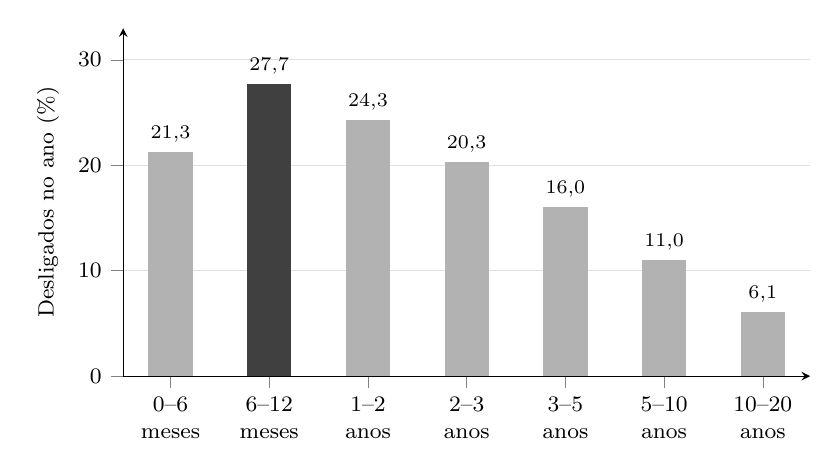
\begin{tikzpicture}
    \begin{axis}[width=\linewidth, height=6.2cm, axis lines=left, tick align=outside,
            ymajorgrids, grid style={black!12}, tick label style={font=\footnotesize},
            label style={font=\footnotesize}, title style={font=\small\bfseries},
            /pgf/number format/use comma, /pgf/number format/1000 sep={.}, width=0.85\textwidth, height=6cm, ymin=0, ymax=33,
            ylabel={Desligados no ano (\%)}, symbolic x coords={f0_6m,f6_12m,f1_2a,f2_3a,f3_5a,f5_10a,f10_20a},
            xtick={f0_6m,f6_12m,f1_2a,f2_3a,f3_5a,f5_10a,f10_20a}, xticklabels={{0--6\\meses},{6--12\\meses},{1--2\\anos},{2--3\\anos},{3--5\\anos},{5--10\\anos},{10--20\\anos}},
            enlarge x limits=0.08, ybar=0pt, bar shift=0pt,
            x tick label style={font=\footnotesize, align=center}]
        \addplot[ybar, bar width=16pt, fill=black!30, draw=none, nodes near coords, nodes near coords style={font=\scriptsize, /pgf/number format/.cd, use comma, fixed, fixed zerofill, precision=1}] coordinates {(f0_6m,21.3)};
        \addplot[ybar, bar width=16pt, fill=black!75, draw=none, nodes near coords, nodes near coords style={font=\scriptsize, /pgf/number format/.cd, use comma, fixed, fixed zerofill, precision=1}] coordinates {(f6_12m,27.7)};
        \addplot[ybar, bar width=16pt, fill=black!30, draw=none, nodes near coords, nodes near coords style={font=\scriptsize, /pgf/number format/.cd, use comma, fixed, fixed zerofill, precision=1}] coordinates {(f1_2a,24.3)};
        \addplot[ybar, bar width=16pt, fill=black!30, draw=none, nodes near coords, nodes near coords style={font=\scriptsize, /pgf/number format/.cd, use comma, fixed, fixed zerofill, precision=1}] coordinates {(f2_3a,20.3)};
        \addplot[ybar, bar width=16pt, fill=black!30, draw=none, nodes near coords, nodes near coords style={font=\scriptsize, /pgf/number format/.cd, use comma, fixed, fixed zerofill, precision=1}] coordinates {(f3_5a,16.0)};
        \addplot[ybar, bar width=16pt, fill=black!30, draw=none, nodes near coords, nodes near coords style={font=\scriptsize, /pgf/number format/.cd, use comma, fixed, fixed zerofill, precision=1}] coordinates {(f5_10a,11.0)};
        \addplot[ybar, bar width=16pt, fill=black!30, draw=none, nodes near coords, nodes near coords style={font=\scriptsize, /pgf/number format/.cd, use comma, fixed, fixed zerofill, precision=1}] coordinates {(f10_20a,6.1)};
    \end{axis}
    \end{tikzpicture}
    \\[4pt]
    {\footnotesize }Fonte: Autoria própria, a partir da camada Gold.
\end{figure}


A \autoref{fig:risco} detalha o risco de desligamento por tempo de casa. O padrão contraria uma expectativa comum: o risco é máximo na faixa de 6 a 12 meses, e não nos primeiros meses, caindo de forma monótona a partir daí. A leitura mais plausível é a interação com o contrato de experiência e com o primeiro ciclo de avaliação: quem passa do primeiro ano tende a ficar.

A tábua de vida de período, calculada para 2024 (último ano em que o desligamento pode ser observado), mostra que cerca de 77\% dos vínculos chegam a completar um ano e menos de 60\% chegam a dois, com mediana de permanência na faixa de dois a três anos. Separando pelas duas lentes do recorte, quem está fora de empresas de TI alcança patamares de permanência mais altos nas faixas longas: 20,3\% atingem a faixa de 5 a 10 anos, contra 15,6\% de quem está em empresa de TI, segunda evidência, independente da remuneração, de que as posições fora do setor são mais estáveis.

O modelo de risco em tempo discreto confirma esse desenho quando as características são comparadas entre pessoas de mesmo perfil no restante. O tempo de casa mantém a forma da \autoref{fig:risco}: contra quem tem até seis meses, a chance de desligamento no ano é 57\% maior entre 6 e 12 meses, 41\% maior entre um e dois anos, igual entre três e cinco e 64\% menor a partir de dez anos. A remuneração é o fator contínuo mais forte: o salário duas vezes maior se associa a 43\% menos chance de desligamento. Entre as áreas, engenharia e pesquisa (razão de chances de 1,90) e gestão e direção (1,53) têm risco maior que desenvolvimento, e suporte e operação, menor (0,73). Mulheres têm 9\% menos chance de desligamento que homens de mesmo perfil, e cada dez anos de idade acrescentam 13\%. Na escolaridade, só mestrado (1,19) e doutorado (1,31) diferem do superior completo, ambos com risco maior, o que é compatível com a saída de profissionais mais qualificados para outras posições, e não com instabilidade. O maior coeficiente, 2,61 para estabelecimentos sem empregados em 31 de dezembro, deve ser lido com cuidado: um estabelecimento que termina o ano sem ninguém é, em boa parte, um que encerrou atividades, de modo que o desligamento é quase consequência da definição.

\section{Pergunta 4: quem ganha menos, e por quê}
\label{sec:resultado-q4}

Pessoas negras e mulheres ganham menos, mas por mecanismos diferentes e com trajetórias opostas: o hiato racial vem de acesso e caiu; o de gênero vem de retorno e surgiu no período.

% Gerado por scripts/gerar_tabelas.py --- não editar à mão.
\begin{table}[htbp]
    \centering
    \caption{Decomposição de Oaxaca-Blinder do hiato salarial}
    \label{tab:hiato}
    \footnotesize
    \renewcommand{\arraystretch}{1.25}
    \begin{tabular}{llrrr}
        \toprule
        \rowcolor{black!8}
        \textbf{Ano} & \textbf{Comparação} & \textbf{Hiato bruto} & \textbf{Parcela explicada (log)} & \textbf{Parcela não explicada (log)} \\
        \midrule
        2007 & Branca vs Parda & 64,0\% & 0,388 & 0,107 \\
        2015 & Branca vs Parda & 42,0\% & 0,274 & 0,077 \\
        2025 & Branca vs Parda & 38,1\% & 0,237 & 0,086 \\
        2007 & Branca vs Preta & 51,1\% & 0,262 & 0,151 \\
        2015 & Branca vs Preta & 41,1\% & 0,194 & 0,151 \\
        2025 & Branca vs Preta & 30,9\% & 0,145 & 0,124 \\
        2007 & Homem vs Mulher & -0,9\% & -0,150 & 0,141 \\
        2015 & Homem vs Mulher & -0,7\% & -0,132 & 0,125 \\
        2025 & Homem vs Mulher & 7,8\% & -0,058 & 0,134 \\
        \bottomrule
    \end{tabular}
    \\[4pt]
    Parcelas em logaritmo da remuneração; referência de Neumark. Fonte: Elaborado pelo autor com dados da RAIS \cite{RAIS2024}.
\end{table}


A \autoref{tab:hiato} apresenta a decomposição de Oaxaca-Blinder para as três comparações calculadas, em três anos da série. Os dois eixos de desigualdade têm estruturas qualitativamente distintas, e é essa distinção, e não a magnitude de cada hiato, o resultado relevante.

No eixo de gênero, o hiato bruto em 2025 é de 7,8\%, e a parcela explicada por características observáveis é negativa. Isso significa que, pelas características que o modelo observa (escolaridade, área, porte, região, tempo de emprego, idade e jornada), as mulheres do setor deveriam ganhar \textit{mais} que os homens. Toda a diferença observada, e um pouco além dela, fica na parcela não explicada: é diferença de retorno às mesmas características, não de características. O resultado converge com o de \citeonline{Dobner2022}, que encontraram o mesmo padrão (atributos produtivos que, sozinhos, fariam as mulheres ganharem mais) na RAIS do Rio Grande do Sul, em todos os setores: não se trata, portanto, de um artefato do recorte deste trabalho.

% Gerado por scripts/gerar_tabelas.py --- não editar à mão.
\begin{figure}[htbp]
    \centering
    \caption{Hiato salarial bruto por raça/cor e por sexo, 2007--2025}
    \label{fig:hiato-serie}
    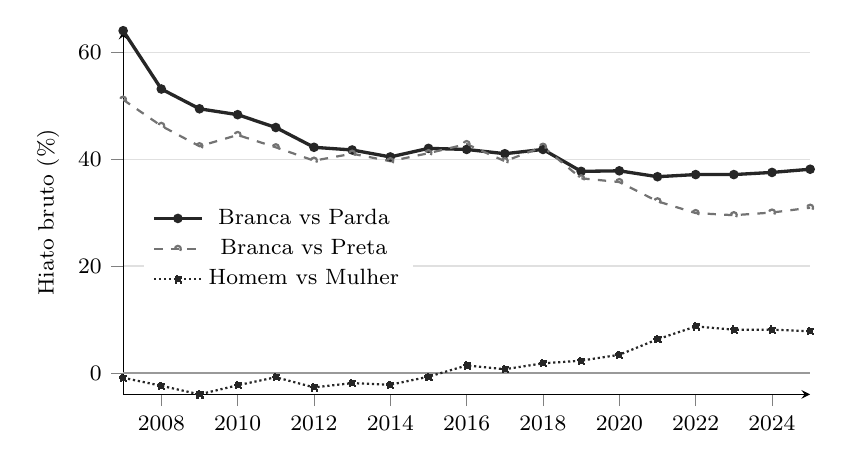
\begin{tikzpicture}
    \begin{axis}[width=\linewidth, height=6.2cm, axis lines=left, tick align=outside,
            ymajorgrids, grid style={black!12}, tick label style={font=\footnotesize},
            label style={font=\footnotesize}, title style={font=\small\bfseries},
            /pgf/number format/use comma, /pgf/number format/1000 sep={.}, width=0.85\textwidth, height=6.2cm, ylabel={Hiato bruto (\%)},
            xmin=2007, xmax=2025, xtick distance=2,
            x tick label style={/pgf/number format/1000 sep={}},
            legend style={font=\footnotesize, at={(0.03,0.40)}, anchor=west, draw=none, fill=white}]
        \addplot[black!40, thin, forget plot] coordinates {(2007,0) (2025,0)};
        \addplot[very thick, black!85, mark=*, mark size=1.1pt] coordinates {(2007,64.0) (2008,53.1) (2009,49.4) (2010,48.3) (2011,45.9) (2012,42.2) (2013,41.7) (2014,40.4) (2015,42.0) (2016,41.8) (2017,41.0) (2018,41.8) (2019,37.7) (2020,37.8) (2021,36.7) (2022,37.1) (2023,37.1) (2024,37.5) (2025,38.1)};
        \addlegendentry{Branca vs Parda}
        \addplot[thick, black!55, dashed, mark=o, mark size=1.1pt] coordinates {(2007,51.1) (2008,46.2) (2009,42.4) (2010,44.5) (2011,42.2) (2012,39.7) (2013,41.0) (2014,39.6) (2015,41.1) (2016,42.8) (2017,39.6) (2018,42.3) (2019,36.4) (2020,35.7) (2021,32.1) (2022,29.9) (2023,29.5) (2024,30.0) (2025,30.9)};
        \addlegendentry{Branca vs Preta}
        \addplot[thick, black!85, densely dotted, mark=square*, mark size=1.1pt] coordinates {(2007,-0.9) (2008,-2.4) (2009,-4.0) (2010,-2.3) (2011,-0.8) (2012,-2.7) (2013,-1.9) (2014,-2.2) (2015,-0.7) (2016,1.4) (2017,0.7) (2018,1.8) (2019,2.3) (2020,3.4) (2021,6.3) (2022,8.7) (2023,8.1) (2024,8.1) (2025,7.8)};
        \addlegendentry{Homem vs Mulher}
    \end{axis}
    \end{tikzpicture}
    \\[4pt]
    {\footnotesize Diferença percentual da remuneração média do primeiro grupo sobre a do segundo; negativo: o segundo grupo ganha mais. }Fonte: Autoria própria, a partir da camada Gold.
\end{figure}


A trajetória, na \autoref{fig:hiato-serie}, mostra que esse hiato é recente. De 2007 a 2015 ele ficou entre $-$4,0\% e $-$0,7\%: as mulheres do setor ganhavam, em média, um pouco mais que os homens. Tornou-se positivo em 2016 e chegou a 8,7\% em 2022. A decomposição mostra o mecanismo. A parcela não explicada ficou entre 0,12 e 0,14 em todo o período; o que mudou foi a parcela explicada, que passou de $-$0,150 para $-$0,058. A penalidade de retorno sempre existiu; o que a encobria era uma vantagem das mulheres em características observáveis, que encolheu. É o mecanismo que \citeonline{BlauKahn2017} descrevem para a queda do hiato nos Estados Unidos, operando no sentido inverso: lá, a escolaridade das mulheres alcançou a dos homens e o hiato caiu; aqui, a vantagem das mulheres se reduziu e o hiato apareceu. A persistência da parcela não explicada, por sua vez, é coerente com o que \citeonline{Goldin2014} e, para o Brasil, \citeonline{Madalozzo2010} encontram: a maior parte da diferença de gênero ocorre entre pessoas da mesma ocupação.

No eixo de raça/cor, a estrutura se inverte. Os hiatos são bem maiores, a maior parte deles é explicada por características (pessoas brancas estão sobre-representadas nas áreas, nos portes e nas regiões que pagam mais) e eles caíram de forma contínua: de 64,0\% para 38,1\% entre brancos e pardos e de 51,1\% para 30,9\% entre brancos e pretos. Quase toda a queda veio da parcela explicada, que recuou de 0,388 para 0,237 e de 0,262 para 0,145, enquanto a não explicada mudou pouco. É desigualdade de acesso (quem chega a quais posições) mais do que de remuneração dentro da mesma posição, e foi o acesso que melhorou. Mesmo depois da queda, os hiatos raciais de TI são cerca de metade dos observados no mercado de trabalho como um todo, em que o rendimento médio de brancos superava em mais de 70\% o de pretos e de pardos em 2021 \cite{IBGE2022Desigualdades}, comparação que vale como ordem de grandeza, porque as duas medidas não são idênticas.

A distinção tem consequência prática direta. Política de equidade salarial dentro da empresa atua sobre a parcela não explicada, e portanto sobre o hiato de gênero; política de acesso (formação, recrutamento, promoção) atua sobre a parcela explicada, e portanto sobre o hiato racial. Tratar os dois eixos com o mesmo instrumento ignora o que a decomposição mostra.

A leitura tem duas ressalvas. A primeira, já registrada na \autoref{subsec:oaxaca}, é que a parcela não explicada é um limite superior para a discriminação, e não uma medida dela. A segunda é que a trajetória do hiato de gênero depende inteiramente da correção do artefato de Rondônia (\autoref{subsec:artefato-ro}): com o funcionalismo estadual contado como programador, o hiato de 2007 aparecia como 19,0\%, e a série contava a história oposta, a de um hiato em queda. Um defeito de declaração em um único órgão bastava para inverter a tendência.

Sobre composição: a participação feminina no estoque de TI caiu de 32,5\% em 2007 para 27,5\% em 2018 e voltou a 30,6\% em 2025; entre os profissionais de ocupação de TI, caiu de 22,9\% para 20,6\%. O setor cresceu 162\% e ficou proporcionalmente menos feminino, o que é um resultado em si. Parte dessa participação, note-se, só aparece por causa da revisão do recorte: a família de estatísticos incorporada tem entre 42\% e 47\% de mulheres, muito acima da média do recorte, evidência de que a delimitação do que se chama ``tecnologia'' afeta a medida de equidade do setor.

\section{Pergunta 5: para onde o mercado vai}
\label{sec:resultado-q5}

O fluxo mensal é previsível por cerca de um ano; o estoque do ano corrente, que a RAIS só publica depois, é estimável com erro próximo de 1\%.

% Gerado por scripts/gerar_tabelas.py --- não editar à mão.
\begin{table}[htbp]
    \centering
    \caption{Desempenho dos modelos na validação de origem móvel}
    \label{tab:previsao}
    \footnotesize
    \renewcommand{\arraystretch}{1.25}
    \begin{tabular}{lrrrr}
        \toprule
        \rowcolor{black!8}
        \textbf{Modelo} & \textbf{Dobras} & \textbf{MAE} & \textbf{RMSE} & \textbf{Ganho sobre o ingênuo} \\
        \midrule
        \texttt{SARIMA(1, 0, 1)(1, 1, 1, 12)} & 5 & 2.558 & 3.339 & 30,6\% \\
        \texttt{SARIMA(2, 0, 1)(1, 1, 1, 12)} & 5 & 2.607 & 3.424 & 29,3\% \\
        \texttt{SARIMA(2, 1, 2)(1, 1, 1, 12)} & 5 & 2.986 & 3.856 & 19,0\% \\
        \texttt{SARIMA(0, 1, 1)(0, 1, 1, 12)} & 5 & 3.119 & 3.926 & 15,4\% \\
        \texttt{SARIMA(1, 1, 1)(0, 1, 1, 12)} & 5 & 3.145 & 3.957 & 14,7\% \\
        \texttt{SARIMA(1, 0, 0)(1, 1, 0, 12)} & 5 & 3.564 & 4.855 & 3,4\% \\
        \texttt{naive sazonal} & 5 & 3.688 & 4.763 & 0,0\% \\
        \bottomrule
    \end{tabular}
    \\[4pt]
    Fonte: Autoria própria, a partir da camada Gold.
\end{table}


A \autoref{tab:previsao} traz o desempenho dos modelos na validação de origem móvel. A especificação vencedora supera o \textit{baseline} ingênuo sazonal em 33\% de erro absoluto médio, o que justifica o modelo: ele erra sensivelmente menos do que repetir o mesmo mês do ano anterior. A margem sobre o \textit{baseline}, porém, varia muito entre as seis especificações testadas (de 33\% a apenas 5\%), e é isso que justifica o piso de comparação: sem ele, a especificação mais fraca pareceria tão aceitável quanto as demais.

O Prophet, modelo previsto na proposta, foi avaliado nas mesmas dobras. Na configuração de tendência mais rígida, superou o \textit{baseline} em 8,3\%, cerca de um quarto do ganho do melhor SARIMA; na configuração padrão e na mais flexível, ficou abaixo do próprio \textit{baseline}. O resultado tem explicação: a série mensal é completa e de sazonalidade estável, o terreno em que a diferenciação sazonal do SARIMA rende mais, e as vantagens do Prophet (tolerância a lacunas e a mudanças de tendência) não se aplicavam. Quanto mais liberdade a tendência recebe, pior o Prophet se sai, o que indica que ele interpreta como mudança de tendência parte do que é ruído do saldo mensal.

O horizonte útil, porém, é curto, e isso corrige a proposta do TCC~1. A previsão mensal de saldo chega ao fim do primeiro ano de projeção com intervalo de predição que cruza o zero: o modelo não distingue, nessa distância, saldo positivo de negativo. Projetar até 2030, como previa a proposta, produziria um número sem conteúdo informativo. O trabalho reporta, portanto, um horizonte de 18 meses, com os intervalos explícitos. No ciclo do CRISP-DM, foi a Avaliação levando de volta ao Entendimento do Negócio: a pergunta deixou de ser apenas ``quanto haverá no futuro'' e passou a incluir ``quanto há agora'', que o \textit{nowcast} a seguir responde.

\subsection{\textit{Nowcast} do estoque}

% Gerado por scripts/gerar_tabelas.py --- não editar à mão.
\begin{table}[htbp]
    \centering
    \caption{\textit{Nowcast} do estoque: erro de cada estimador com cada ano retido, 2014--2025}
    \label{tab:nowcast}
    \footnotesize
    \renewcommand{\arraystretch}{1.25}
    \begin{tabular}{lrrrr}
        \toprule
        \rowcolor{black!8}
        \textbf{Estimador} & \textbf{Erro médio} & \textbf{Erro mediano} & \textbf{Maior erro (ano)} & \textbf{Erro em 2025} \\
        \midrule
        razão mediana & 1,07\% & 0,92\% & -2,8\% (2022) & -0,90\% \\
        regressão OLS & 1,40\% & 1,16\% & 3,0\% (2017) & -0,88\% \\
        identidade (delta = fluxo) & 1,59\% & 1,39\% & -4,4\% (2022) & -1,43\% \\
        ingênuo (sem mudança) & 5,10\% & 3,79\% & -16,2\% (2021) & -3,67\% \\
        \bottomrule
    \end{tabular}
    \\[4pt]
    Erros em \% do estoque observado; médio e mediano em valor absoluto. Cada ano é estimado só com os anteriores. Fonte: Elaborado pelo autor com dados da RAIS e do CAGED \cite{RAIS2024, CAGED2024}.
\end{table}



A limitação de horizonte da previsão mensal contrasta com um resultado bem mais forte na estimação do presente. O estoque do ano corrente é desconhecido até a RAIS ser publicada no ano seguinte, mas o CAGED já divulgou parte do fluxo. A \autoref{tab:nowcast} e a \autoref{fig:nowcast-anos} mostram o teste feito: cada ano de 2014 a 2025 foi estimado sem os dados daquele ano e dos seguintes, como se estivesse em curso, e comparado com o estoque que a RAIS publicou depois.

% Gerado por scripts/gerar_tabelas.py --- não editar à mão.
\begin{figure}[htbp]
    \centering
    \caption{Erro do \textit{nowcast} em cada ano retido, 2014--2025}
    \label{fig:nowcast-anos}
    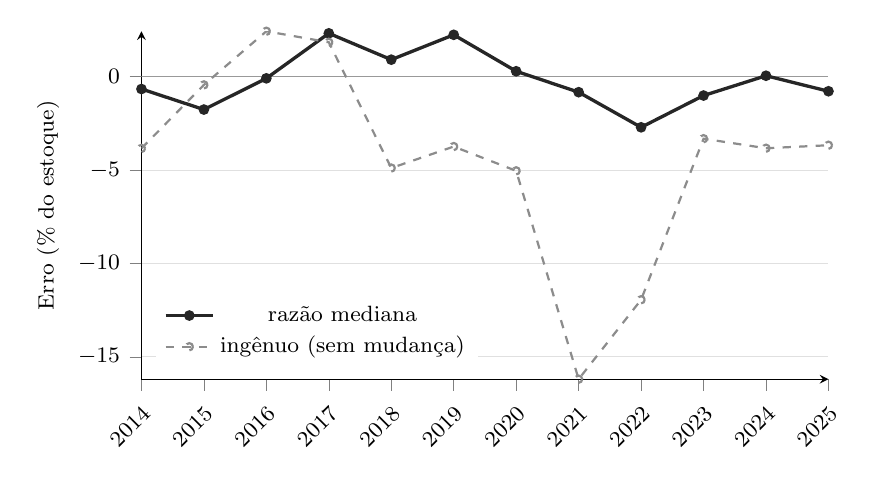
\begin{tikzpicture}
    \begin{axis}[width=\linewidth, height=6.2cm, axis lines=left, tick align=outside,
            ymajorgrids, grid style={black!12}, tick label style={font=\footnotesize},
            label style={font=\footnotesize}, title style={font=\small\bfseries},
            /pgf/number format/use comma, /pgf/number format/1000 sep={.}, width=0.85\textwidth, height=6cm, ylabel={Erro (\% do estoque)},
            xmin=2014, xmax=2025, xtick distance=1,
            x tick label style={/pgf/number format/1000 sep={}, rotate=45, anchor=north east},
            legend style={font=\footnotesize, at={(0.02,0.03)}, anchor=south west, draw=none, fill=white}]
        \addplot[black!40, thin, forget plot] coordinates {(2014,0) (2025,0)};
        \addplot[very thick, black!85, mark=*, mark size=1.3pt] coordinates {(2014,-0.66) (2015,-1.76) (2016,-0.09) (2017,2.32) (2018,0.91) (2019,2.24) (2020,0.29) (2021,-0.83) (2022,-2.71) (2023,-1.01) (2024,0.05) (2025,-0.78)};
        \addlegendentry{razão mediana}
        \addplot[thick, black!45, dashed, mark=o, mark size=1.3pt] coordinates {(2014,-3.84) (2015,-0.44) (2016,2.43) (2017,1.84) (2018,-4.89) (2019,-3.74) (2020,-5.04) (2021,-16.19) (2022,-11.94) (2023,-3.32) (2024,-3.83) (2025,-3.67)};
        \addlegendentry{ingênuo (sem mudança)}
    \end{axis}
    \end{tikzpicture}
    \\[4pt]
    {\footnotesize Erro positivo: o estimador superestimou o estoque. }Fonte: Autoria própria, a partir da camada Gold.
\end{figure}


O melhor estimador, a razão mediana histórica entre a variação do estoque e o saldo do CAGED, erra em média 1,1\% (a mediana é de 0,9\%), contra 1,6\% da identidade direta e 5,1\% do estimador ingênuo, que supõe estoque constante. Em onze dos doze anos o erro ficou abaixo de 2,3\%, e o maior foi o de 2022, de 2,8\%, ano em que o estoque cresceu mais do que o saldo do CAGED indicava. A razão supera a identidade porque a variação do estoque e o saldo do fluxo não andam de um para um (\autoref{sec:coerencia-bases}), e a razão incorpora essa relação histórica. No último ano retido, 2025, os três estimadores apoiados no fluxo erraram entre 0,88\% e 1,43\%.

Antes da correção do artefato de Rondônia, o erro médio era de 2,1\%, e os dois piores anos eram 2018 e 2022, atribuídos então à diferença de cobertura entre as bases. Eram dois dos anos em que o funcionalismo estadual entrou no estoque da RAIS sem nunca passar pelo CAGED: parte do que parecia limite do método era defeito do dado.

Aplicado ao ano corrente, com oito meses de CAGED já publicados, o estimador projeta 1.371.853 vínculos em 31 de dezembro de 2026, um crescimento de 0,8\% sobre 2025; a margem, de cerca de 32 mil vínculos, vai de uma queda de 1,6\% a uma alta de 3,1\%. A previsão de fluxo aponta na mesma direção: o saldo acumulado esperado para os doze meses seguintes é de 14,6 mil vagas, com intervalo que vai de $-$34 mil a $+$62 mil. Os dois resultados confirmam a desaceleração posterior a 2022. Na prática, enquanto a previsão de fluxo a doze meses é incerta, a estimativa do estoque corrente erra pouco na maior parte dos anos, porque se apoia em informação já observada em lugar de extrapolação.

Essa assimetria (previsão de futuro incerta, estimação de presente bem mais precisa) é a mesma que a literatura de \textit{nowcasting} explora para o PIB \cite{Giannone2008, Banbura2013}, aplicada aqui ao emprego, e é o resultado de modelagem mais útil do trabalho: em bases com defasagem de publicação, estimar o que já aconteceu e ainda não foi divulgado rende mais do que prever o que não aconteceu.

\section{O \textit{dashboard} entregue}

A camada de apresentação, descrita na \autoref{sec:apresentacao}, foi organizada pelas cinco perguntas de pesquisa, e não pela origem do dado, correção de uma primeira versão em que as abas, organizadas por base, mostravam gráficos corretos que não chegavam a uma conclusão. Um gráfico só permanece em uma página se sustenta a resposta daquela pergunta; os recortes que não sustentam uma resposta, como o saldo por setor e por ocupação, saíram do painel, que ficou com a visão geral, as cinco perguntas e as páginas de análise. A \autoref{fig:dashboard}(a) mostra a abertura de uma página de pergunta: a pergunta, os filtros e os indicadores, antes dos gráficos.

O filtro de território torna a interface um instrumento de verificação, e não só de leitura. A \autoref{fig:dashboard}(b) mostra o efeito de retirar São Paulo do recorte sobre o mapa: o estado excluído sai da escala de cor, que passa a distinguir os demais, e os indicadores são recalculados para o recorte. Do mesmo modo, a análise de sensibilidade sobre São Paulo apresentada na \autoref{sec:resultado-q2} pode ser refeita em qualquer gráfico do painel.

\begin{figure}[htbp]
    \centering
    \caption{O \textit{dashboard}: página de uma pergunta de pesquisa (a) e mapa sem São Paulo no recorte (b)}
    \label{fig:dashboard}
    \begin{minipage}[t]{0.495\textwidth}
        \centering
        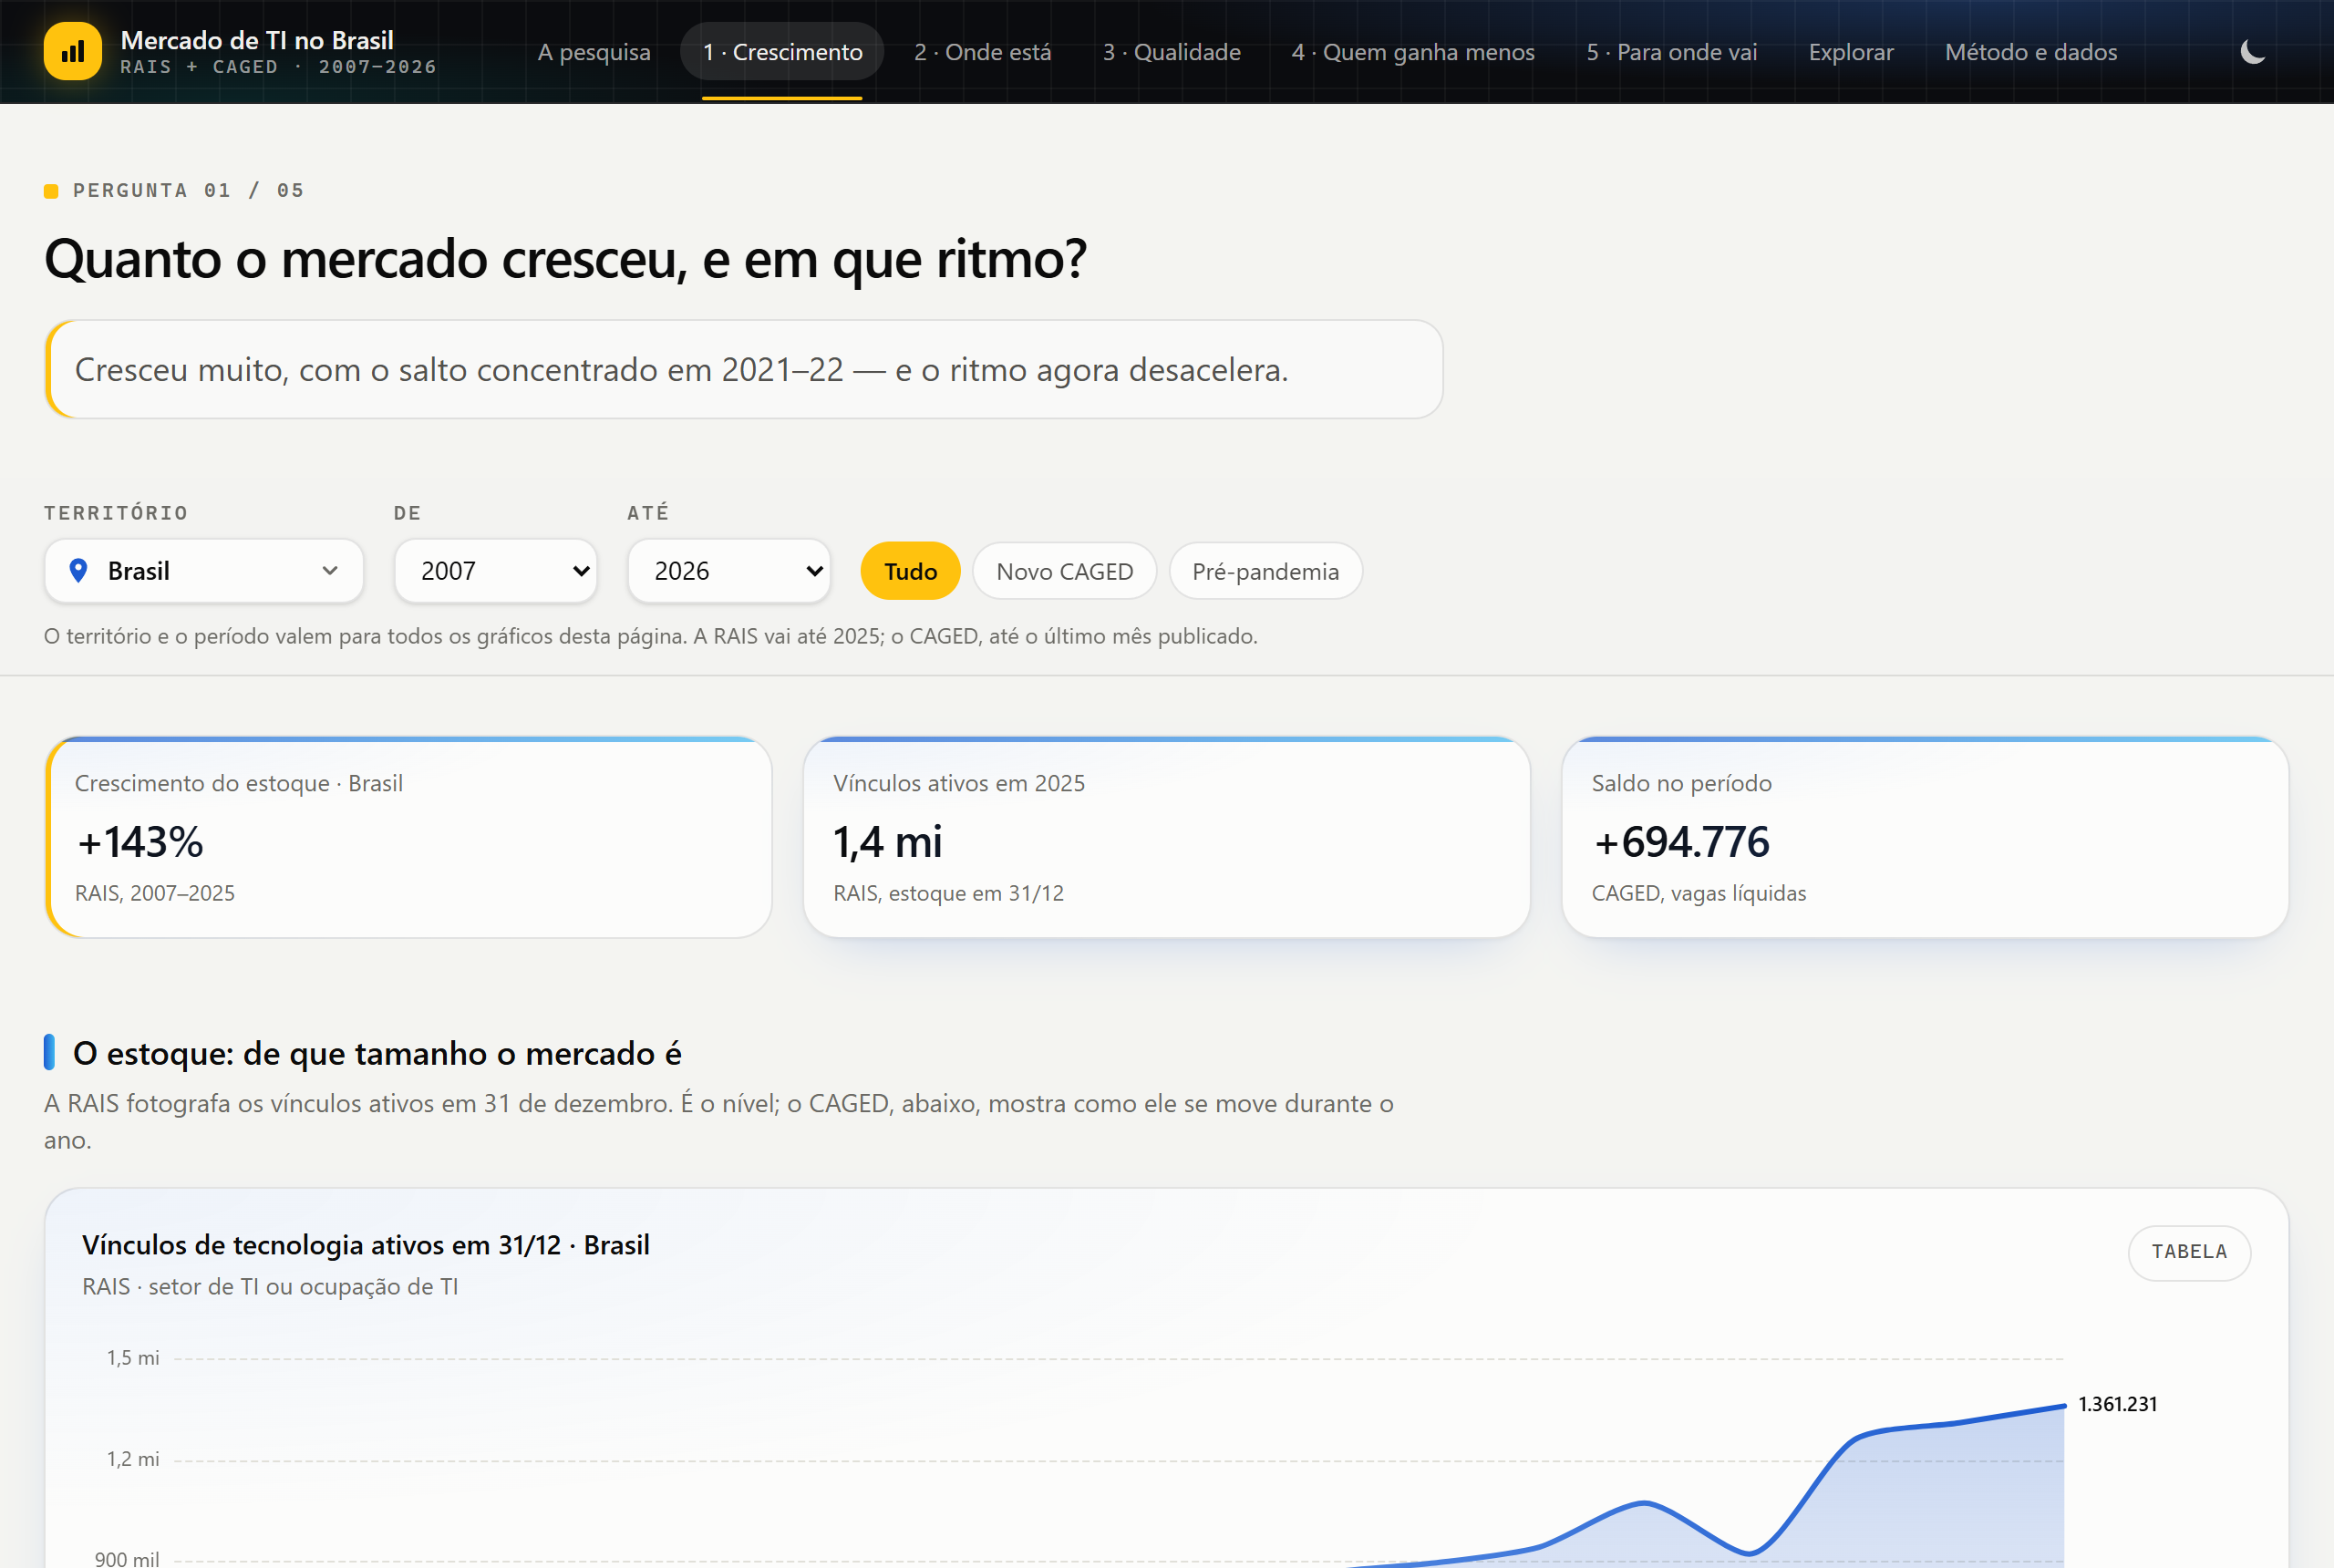
\includegraphics[width=\linewidth]{figuras/dashboard-pergunta.png}\\[2pt]
        {\footnotesize (a) Abertura da página da primeira pergunta}
    \end{minipage}\hfill
    \begin{minipage}[t]{0.495\textwidth}
        \centering
        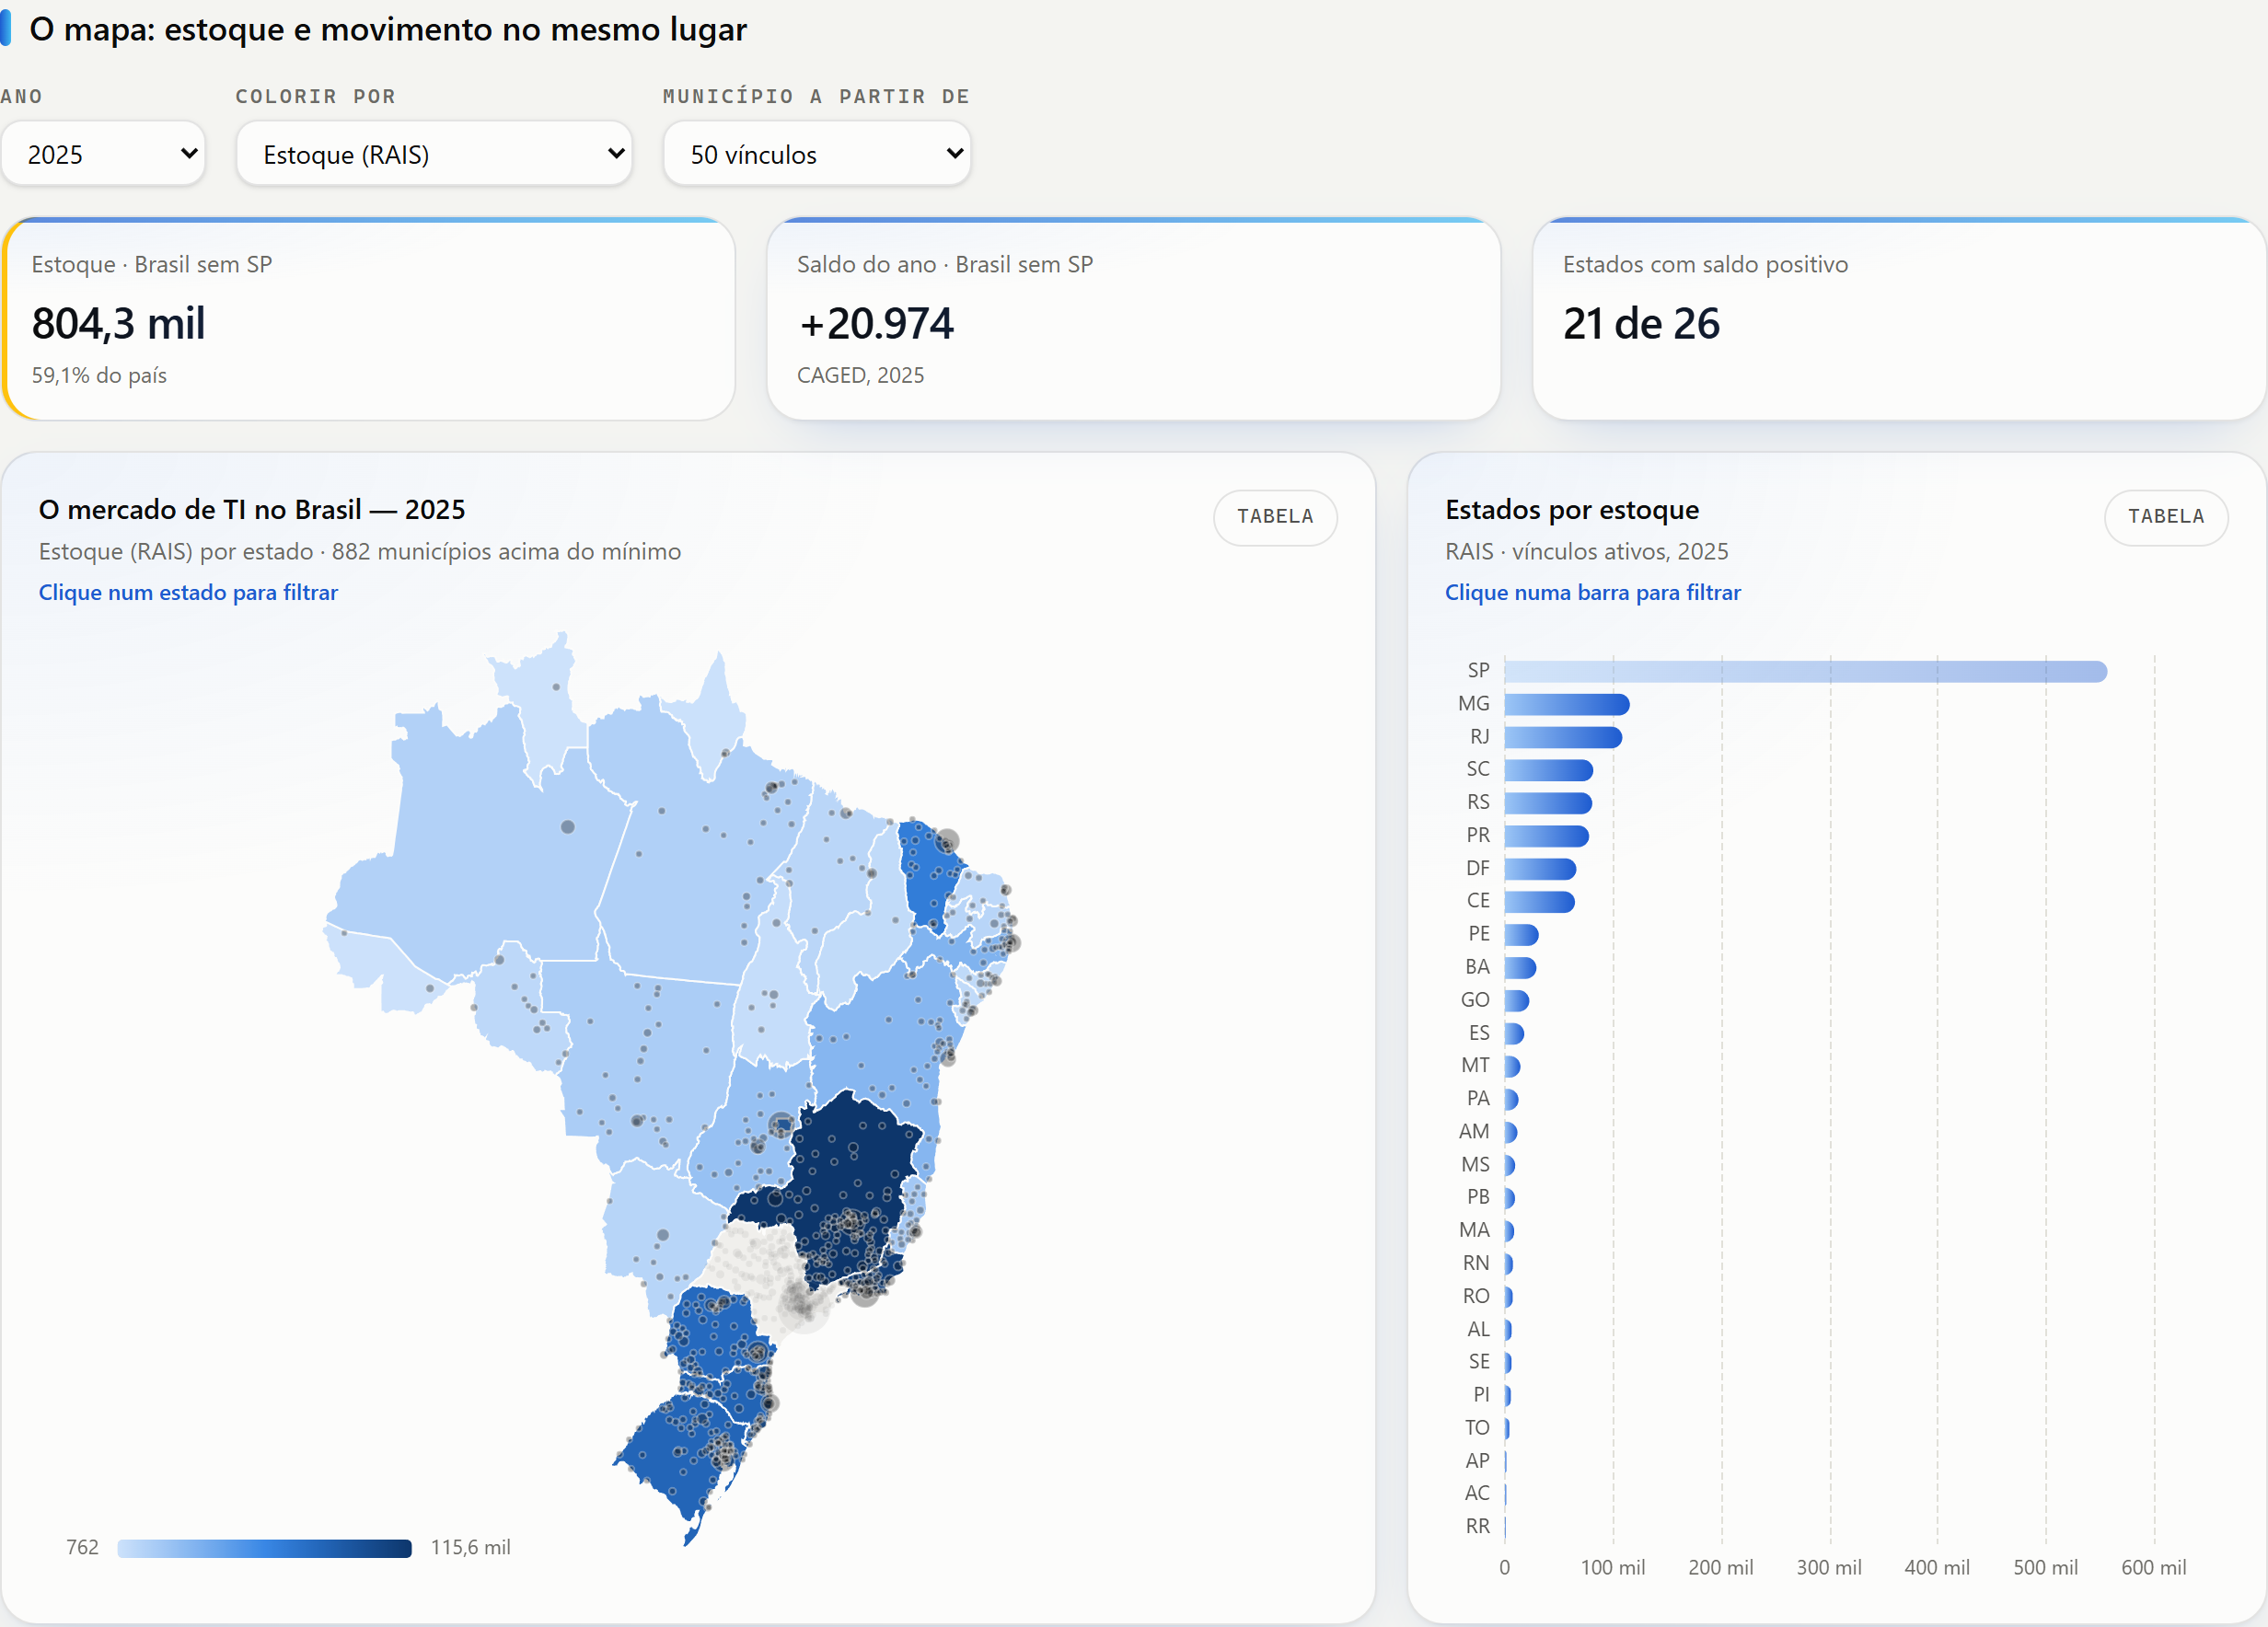
\includegraphics[width=\linewidth]{figuras/dashboard-mapa-filtro.png}\\[2pt]
        {\footnotesize (b) Mapa e \textit{ranking} de estados sem São Paulo}
    \end{minipage}
    \\[4pt]
    Fonte: Elaborado pelo autor.
\end{figure}
